\documentclass[a4paper]{report}

%%%%%%%%%%%%%%%%%%%%%%%%%%%%%%%%%
% PACKAGE IMPORTS
%%%%%%%%%%%%%%%%%%%%%%%%%%%%%%%%%


\usepackage[tmargin=2cm,rmargin=1in,lmargin=1in,margin=0.85in,bmargin=2cm,footskip=.2in]{geometry}
\usepackage[onehalfspacing]{setspace}
\usepackage{graphicx}
\usepackage{float}
% 以下包可根据需要启用
\usepackage{icomma}
\usepackage{nicematrix}
\usepackage[english]{babel}
\usepackage{csquotes}
\usepackage[T1]{fontenc} % 注意：可能与xeCJK冲突
\usepackage[locale = US,space-before-unit=true,per-mode = symbol]{siunitx}
\usepackage{placeins}
\usepackage{booktabs}
\usepackage{multirow}
\usepackage{arydshln}
\usepackage[natbib,abbreviate=true,doi=false,style=numeric-comp,giveninits=true,sorting=none]{biblatex}
\usepackage{amsmath,amsfonts,amsthm,amssymb,mathtools}
\usepackage[varbb]{newpxmath}
\usepackage{xfrac}
\usepackage{xeCJK}
\IfFontExistsTF{Source Han Serif}
    {\setCJKmainfont{Source Han Serif}}
    {\setCJKmainfont{FandolSong-Regular.otf}[BoldFont=FandolSong-Bold.otf]}
\usepackage[makeroom]{cancel}
\usepackage{mathtools}
\usepackage{bookmark}
\usepackage{enumitem}
\usepackage{hyperref,theoremref}
\hypersetup{
	pdftitle={Assignment},
	colorlinks=true, linkcolor=whusakura, urlcolor=whusakura,
	bookmarksnumbered=true,
	bookmarksopen=true
}
\usepackage[most,many,breakable]{tcolorbox}
\usepackage{xcolor}
\usepackage{varwidth}
\usepackage{varwidth}
\usepackage{etoolbox}
\usepackage{makecell}
%\usepackage{authblk}
\usepackage{nameref}
\usepackage{multicol,array}
\usepackage{tikz-cd}
\usepackage{pgfplots}
\usepgfplotslibrary{groupplots}
\usepackage[ruled,vlined,linesnumbered]{algorithm2e}
\usepackage{comment} % enables the use of multi-line comments (\ifx \fi)
\usepackage{import}
\usepackage{xifthen}
\usepackage{pdfpages}

\newcommand\mycommfont[1]{\footnotesize\ttfamily\textcolor{blue}{#1}}
\SetCommentSty{mycommfont}
\newcommand{\incfig}[1]{%
    \def\svgwidth{\columnwidth}
    \import{./figures/}{#1.pdf_tex}
}

\usepackage{tikzsymbols}
\renewcommand\qedsymbol{$\Laughey$}


%\usepackage{import}
%\usepackage{xifthen}
%\usepackage{pdfpages}
%\usepackage{transparent}


%%%%%%%%%%%%%%%%%%%%%%%%%%%%%%
% SELF MADE COLORS
%%%%%%%%%%%%%%%%%%%%%%%%%%%%%%



\definecolor{whusakura}{RGB}{248, 163, 188}
\definecolor{myg}{RGB}{56, 140, 70}
\definecolor{myb}{RGB}{45, 111, 177}
\definecolor{myr}{RGB}{199, 68, 64}
\definecolor{mytheorembg}{HTML}{F2F2F9}
\definecolor{mytheoremfr}{HTML}{00007B}
\definecolor{mylenmabg}{HTML}{FFFAF8}
\definecolor{mylenmafr}{HTML}{983b0f}
\definecolor{mypropbg}{HTML}{f2fbfc}
\definecolor{mypropfr}{HTML}{191971}
\definecolor{myexamplebg}{HTML}{F2FBF8}
\definecolor{myexamplefr}{HTML}{88D6D1}
\definecolor{myexampleti}{HTML}{2A7F7F}
\definecolor{mydefinitbg}{HTML}{E5E5FF}
\definecolor{mydefinitfr}{HTML}{3F3FA3}
\definecolor{notesgreen}{RGB}{0,162,0}
\definecolor{myp}{RGB}{197, 92, 212}
\definecolor{mygr}{HTML}{2C3338}
\definecolor{myred}{RGB}{127,0,0}
\definecolor{myyellow}{RGB}{169,121,69}
\definecolor{myexercisebg}{HTML}{F2FBF8}
\definecolor{myexercisefg}{HTML}{88D6D1}


%%%%%%%%%%%%%%%%%%%%%%%%%%%%
% TCOLORBOX SETUPS
%%%%%%%%%%%%%%%%%%%%%%%%%%%%

\setlength{\parindent}{1cm}
%================================
% THEOREM BOX
%================================

\tcbuselibrary{theorems,skins,hooks}
\newtcbtheorem[number within=section]{Theorem}{Theorem}
{%
	enhanced,
	breakable,
	colback = mytheorembg,
	frame hidden,
	boxrule = 0sp,
	borderline west = {2pt}{0pt}{mytheoremfr},
	sharp corners,
	detach title,
	before upper = \tcbtitle\par\smallskip,
	coltitle = mytheoremfr,
	fonttitle = \bfseries\sffamily,
	description font = \mdseries,
	separator sign none,
	segmentation style={solid, mytheoremfr},
}
{th}

\tcbuselibrary{theorems,skins,hooks}
\newtcbtheorem[number within=chapter]{theorem}{Theorem}
{%
	enhanced,
	breakable,
	colback = mytheorembg,
	frame hidden,
	boxrule = 0sp,
	borderline west = {2pt}{0pt}{mytheoremfr},
	sharp corners,
	detach title,
	before upper = \tcbtitle\par\smallskip,
	coltitle = mytheoremfr,
	fonttitle = \bfseries\sffamily,
	description font = \mdseries,
	separator sign none,
	segmentation style={solid, mytheoremfr},
}
{th}


\tcbuselibrary{theorems,skins,hooks}
\newtcolorbox{Theoremcon}
{%
	enhanced
	,breakable
	,colback = mytheorembg
	,frame hidden
	,boxrule = 0sp
	,borderline west = {2pt}{0pt}{mytheoremfr}
	,sharp corners
	,description font = \mdseries
	,separator sign none
}

%================================
% Corollery
%================================
\tcbuselibrary{theorems,skins,hooks}
\newtcbtheorem[number within=section]{Corollary}{Corollary}
{%
	enhanced
	,breakable
	,colback = myp!10
	,frame hidden
	,boxrule = 0sp
	,borderline west = {2pt}{0pt}{myp!85!black}
	,sharp corners
	,detach title
	,before upper = \tcbtitle\par\smallskip
	,coltitle = myp!85!black
	,fonttitle = \bfseries\sffamily
	,description font = \mdseries
	,separator sign none
	,segmentation style={solid, myp!85!black}
}
{th}
\tcbuselibrary{theorems,skins,hooks}
\newtcbtheorem[number within=chapter]{corollary}{Corollary}
{%
	enhanced
	,breakable
	,colback = myp!10
	,frame hidden
	,boxrule = 0sp
	,borderline west = {2pt}{0pt}{myp!85!black}
	,sharp corners
	,detach title
	,before upper = \tcbtitle\par\smallskip
	,coltitle = myp!85!black
	,fonttitle = \bfseries\sffamily
	,description font = \mdseries
	,separator sign none
	,segmentation style={solid, myp!85!black}
}
{th}


%================================
% LENMA
%================================

\tcbuselibrary{theorems,skins,hooks}
\newtcbtheorem[number within=section]{Lenma}{Lenma}
{%
	enhanced,
	breakable,
	colback = mylenmabg,
	frame hidden,
	boxrule = 0sp,
	borderline west = {2pt}{0pt}{mylenmafr},
	sharp corners,
	detach title,
	before upper = \tcbtitle\par\smallskip,
	coltitle = mylenmafr,
	fonttitle = \bfseries\sffamily,
	description font = \mdseries,
	separator sign none,
	segmentation style={solid, mylenmafr},
}
{th}

\tcbuselibrary{theorems,skins,hooks}
\newtcbtheorem[number within=chapter]{lenma}{Lenma}
{%
	enhanced,
	breakable,
	colback = mylenmabg,
	frame hidden,
	boxrule = 0sp,
	borderline west = {2pt}{0pt}{mylenmafr},
	sharp corners,
	detach title,
	before upper = \tcbtitle\par\smallskip,
	coltitle = mylenmafr,
	fonttitle = \bfseries\sffamily,
	description font = \mdseries,
	separator sign none,
	segmentation style={solid, mylenmafr},
}
{th}


%================================
% PROPOSITION
%================================

\tcbuselibrary{theorems,skins,hooks}
\newtcbtheorem[number within=section]{Prop}{Proposition}
{%
	enhanced,
	breakable,
	colback = mypropbg,
	frame hidden,
	boxrule = 0sp,
	borderline west = {2pt}{0pt}{mypropfr},
	sharp corners,
	detach title,
	before upper = \tcbtitle\par\smallskip,
	coltitle = mypropfr,
	fonttitle = \bfseries\sffamily,
	description font = \mdseries,
	separator sign none,
	segmentation style={solid, mypropfr},
}
{th}

\tcbuselibrary{theorems,skins,hooks}
\newtcbtheorem[number within=chapter]{prop}{Proposition}
{%
	enhanced,
	breakable,
	colback = mypropbg,
	frame hidden,
	boxrule = 0sp,
	borderline west = {2pt}{0pt}{mypropfr},
	sharp corners,
	detach title,
	before upper = \tcbtitle\par\smallskip,
	coltitle = mypropfr,
	fonttitle = \bfseries\sffamily,
	description font = \mdseries,
	separator sign none,
	segmentation style={solid, mypropfr},
}
{th}


%================================
% CLAIM
%================================

\tcbuselibrary{theorems,skins,hooks}
\newtcbtheorem[number within=section]{claim}{Claim}
{%
	enhanced
	,breakable
	,colback = myg!10
	,frame hidden
	,boxrule = 0sp
	,borderline west = {2pt}{0pt}{myg}
	,sharp corners
	,detach title
	,before upper = \tcbtitle\par\smallskip
	,coltitle = myg!85!black
	,fonttitle = \bfseries\sffamily
	,description font = \mdseries
	,separator sign none
	,segmentation style={solid, myg!85!black}
}
{th}



%================================
% Exercise
%================================

\tcbuselibrary{theorems,skins,hooks}
\newtcbtheorem[number within=section]{Exercise}{Exercise}
{%
	enhanced,
	breakable,
	colback = myexercisebg,
	frame hidden,
	boxrule = 0sp,
	borderline west = {2pt}{0pt}{myexercisefg},
	sharp corners,
	detach title,
	before upper = \tcbtitle\par\smallskip,
	coltitle = myexercisefg,
	fonttitle = \bfseries\sffamily,
	description font = \mdseries,
	separator sign none,
	segmentation style={solid, myexercisefg},
}
{th}

\tcbuselibrary{theorems,skins,hooks}
\newtcbtheorem[number within=chapter]{exercise}{Exercise}
{%
	enhanced,
	breakable,
	colback = myexercisebg,
	frame hidden,
	boxrule = 0sp,
	borderline west = {2pt}{0pt}{myexercisefg},
	sharp corners,
	detach title,
	before upper = \tcbtitle\par\smallskip,
	coltitle = myexercisefg,
	fonttitle = \bfseries\sffamily,
	description font = \mdseries,
	separator sign none,
	segmentation style={solid, myexercisefg},
}
{th}

%================================
% EXAMPLE BOX
%================================

\newtcbtheorem[number within=section]{Example}{Example}
{%
	colback = myexamplebg
	,breakable
	,colframe = myexamplefr
	,coltitle = myexampleti
	,boxrule = 1pt
	,sharp corners
	,detach title
	,before upper=\tcbtitle\par\smallskip
	,fonttitle = \bfseries
	,description font = \mdseries
	,separator sign none
	,description delimiters parenthesis
}
{ex}

\newtcbtheorem[number within=chapter]{example}{Example}
{%
	colback = myexamplebg
	,breakable
	,colframe = myexamplefr
	,coltitle = myexampleti
	,boxrule = 1pt
	,sharp corners
	,detach title
	,before upper=\tcbtitle\par\smallskip
	,fonttitle = \bfseries
	,description font = \mdseries
	,separator sign none
	,description delimiters parenthesis
}
{ex}

%================================
% DEFINITION BOX
%================================

\newtcbtheorem[number within=section]{Definition}{Definition}{enhanced,
	before skip=2mm,after skip=2mm, colback=red!5,colframe=red!80!black,boxrule=0.5mm,
	attach boxed title to top left={xshift=1cm,yshift*=1mm-\tcboxedtitleheight}, varwidth boxed title*=-3cm,
	boxed title style={frame code={
					\path[fill=tcbcolback]
					([yshift=-1mm,xshift=-1mm]frame.north west)
					arc[start angle=0,end angle=180,radius=1mm]
					([yshift=-1mm,xshift=1mm]frame.north east)
					arc[start angle=180,end angle=0,radius=1mm];
					\path[left color=tcbcolback!60!black,right color=tcbcolback!60!black,
						middle color=tcbcolback!80!black]
					([xshift=-2mm]frame.north west) -- ([xshift=2mm]frame.north east)
					[rounded corners=1mm]-- ([xshift=1mm,yshift=-1mm]frame.north east)
					-- (frame.south east) -- (frame.south west)
					-- ([xshift=-1mm,yshift=-1mm]frame.north west)
					[sharp corners]-- cycle;
				},interior engine=empty,
		},
	fonttitle=\bfseries,
	title={#2},#1}{def}
\newtcbtheorem[number within=chapter]{definition}{Definition}{enhanced,
	before skip=2mm,after skip=2mm, colback=red!5,colframe=red!80!black,boxrule=0.5mm,
	attach boxed title to top left={xshift=1cm,yshift*=1mm-\tcboxedtitleheight}, varwidth boxed title*=-3cm,
	boxed title style={frame code={
					\path[fill=tcbcolback]
					([yshift=-1mm,xshift=-1mm]frame.north west)
					arc[start angle=0,end angle=180,radius=1mm]
					([yshift=-1mm,xshift=1mm]frame.north east)
					arc[start angle=180,end angle=0,radius=1mm];
					\path[left color=tcbcolback!60!black,right color=tcbcolback!60!black,
						middle color=tcbcolback!80!black]
					([xshift=-2mm]frame.north west) -- ([xshift=2mm]frame.north east)
					[rounded corners=1mm]-- ([xshift=1mm,yshift=-1mm]frame.north east)
					-- (frame.south east) -- (frame.south west)
					-- ([xshift=-1mm,yshift=-1mm]frame.north west)
					[sharp corners]-- cycle;
				},interior engine=empty,
		},
	fonttitle=\bfseries,
	title={#2},#1}{def}



%================================
% Solution BOX
%================================

\makeatletter
\newtcbtheorem{question}{Question}{enhanced,
	breakable,
	colback=white,
	colframe=myb!80!black,
	attach boxed title to top left={yshift*=-\tcboxedtitleheight},
	fonttitle=\bfseries,
	title={#2},
	boxed title size=title,
	boxed title style={%
			sharp corners,
			rounded corners=northwest,
			colback=tcbcolframe,
			boxrule=0pt,
		},
	underlay boxed title={%
			\path[fill=tcbcolframe] (title.south west)--(title.south east)
			to[out=0, in=180] ([xshift=5mm]title.east)--
			(title.center-|frame.east)
			[rounded corners=\kvtcb@arc] |-
			(frame.north) -| cycle;
		},
	#1
}{def}
\makeatother

%================================
% SOLUTION BOX
%================================

\makeatletter
\newtcolorbox{solution}{enhanced,
	breakable,
	colback=white,
	colframe=myg!80!black,
	attach boxed title to top left={yshift*=-\tcboxedtitleheight},
	title=Solution,
	boxed title size=title,
	boxed title style={%
			sharp corners,
			rounded corners=northwest,
			colback=tcbcolframe,
			boxrule=0pt,
		},
	underlay boxed title={%
			\path[fill=tcbcolframe] (title.south west)--(title.south east)
			to[out=0, in=180] ([xshift=5mm]title.east)--
			(title.center-|frame.east)
			[rounded corners=\kvtcb@arc] |-
			(frame.north) -| cycle;
		},
}
\makeatother

%================================
% Question BOX
%================================

\makeatletter
\newtcbtheorem{qstion}{Question}{enhanced,
	breakable,
	colback=white,
	colframe=mygr,
	attach boxed title to top left={yshift*=-\tcboxedtitleheight},
	fonttitle=\bfseries,
	title={#2},
	boxed title size=title,
	boxed title style={%
			sharp corners,
			rounded corners=northwest,
			colback=tcbcolframe,
			boxrule=0pt,
		},
	underlay boxed title={%
			\path[fill=tcbcolframe] (title.south west)--(title.south east)
			to[out=0, in=180] ([xshift=5mm]title.east)--
			(title.center-|frame.east)
			[rounded corners=\kvtcb@arc] |-
			(frame.north) -| cycle;
		},
	#1
}{def}
\makeatother

\newtcbtheorem[number within=chapter]{wconc}{Wrong Concept}{
	breakable,
	enhanced,
	colback=white,
	colframe=myr,
	arc=0pt,
	outer arc=0pt,
	fonttitle=\bfseries\sffamily\large,
	colbacktitle=myr,
	attach boxed title to top left={},
	boxed title style={
			enhanced,
			skin=enhancedfirst jigsaw,
			arc=3pt,
			bottom=0pt,
			interior style={fill=myr}
		},
	#1
}{def}



%================================
% NOTE BOX
%================================

\usetikzlibrary{backgrounds, 3d, arrows, calc, quotes, shadows.blur, arrows.meta, decorations.pathreplacing, decorations.markings}
\usetikzlibrary{tikzmark, fit, shapes.geometric, positioning, shapes.arrows, patterns}
\tcbuselibrary{skins}
\newtcolorbox{note}[1][]{%
	enhanced jigsaw,
	colback=gray!20!white,%
	colframe=gray!80!black,
	size=small,
	boxrule=1pt,
	title=\textbf{Note:-},
	halign title=flush center,
	coltitle=black,
	breakable,
	drop shadow=black!50!white,
	attach boxed title to top left={xshift=1cm,yshift=-\tcboxedtitleheight/2,yshifttext=-\tcboxedtitleheight/2},
	minipage boxed title=1.5cm,
	boxed title style={%
			colback=white,
			size=fbox,
			boxrule=1pt,
			boxsep=2pt,
			underlay={%
					\coordinate (dotA) at ($(interior.west) + (-0.5pt,0)$);
					\coordinate (dotB) at ($(interior.east) + (0.5pt,0)$);
					\begin{scope}
						\clip (interior.north west) rectangle ([xshift=3ex]interior.east);
						\filldraw [white, blur shadow={shadow opacity=60, shadow yshift=-.75ex}, rounded corners=2pt] (interior.north west) rectangle (interior.south east);
					\end{scope}
					\begin{scope}[gray!80!black]
						\fill (dotA) circle (2pt);
						\fill (dotB) circle (2pt);
					\end{scope}
				},
		},
	#1,
}

%%%%%%%%%%%%%%%%%%%%%%%%%%%%%%
% SELF MADE COMMANDS
%%%%%%%%%%%%%%%%%%%%%%%%%%%%%%


\newcommand{\thm}[2]{\begin{Theorem}{#1}{}#2\end{Theorem}}
\newcommand{\cor}[2]{\begin{Corollary}{#1}{}#2\end{Corollary}}
\newcommand{\mlenma}[2]{\begin{Lenma}{#1}{}#2\end{Lenma}}
\newcommand{\mprop}[2]{\begin{Prop}{#1}{}#2\end{Prop}}
\newcommand{\clm}[3]{\begin{claim}{#1}{#2}#3\end{claim}}
\newcommand{\wc}[2]{\begin{wconc}{#1}{}\setlength{\parindent}{1cm}#2\end{wconc}}
\newcommand{\thmcon}[1]{\begin{Theoremcon}{#1}\end{Theoremcon}}
\newcommand{\ex}[2]{\begin{Example}{#1}{}#2\end{Example}}
\newcommand{\dfn}[2]{\begin{Definition}[colbacktitle=red!75!black]{#1}{}#2\end{Definition}}
\newcommand{\dfnc}[2]{\begin{definition}[colbacktitle=red!75!black]{#1}{}#2\end{definition}}
\newcommand{\qs}[2]{\begin{question}{#1}{}#2\end{question}}
\newcommand{\pf}[2]{\begin{myproof}[#1]#2\end{myproof}}
\newcommand{\nt}[1]{\begin{note}#1\end{note}}

\newcommand*\circled[1]{\tikz[baseline=(char.base)]{
		\node[shape=circle,draw,inner sep=1pt] (char) {#1};}}
\newcommand\getcurrentref[1]{%
	\ifnumequal{\value{#1}}{0}
	{??}
	{\the\value{#1}}%
}
\newcommand{\getCurrentSectionNumber}{\getcurrentref{section}}
\newenvironment{myproof}[1][\proofname]{%
	\proof[\bfseries #1: ]%
}{\endproof}

\newcommand{\mclm}[2]{\begin{myclaim}[#1]#2\end{myclaim}}
\newenvironment{myclaim}[1][\claimname]{\proof[\bfseries #1: ]}{}

\newcounter{mylabelcounter}

\makeatletter
\newcommand{\setword}[2]{%
	\phantomsection
	#1\def\@currentlabel{\unexpanded{#1}}\label{#2}%
}
\makeatother




\tikzset{
	symbol/.style={
			draw=none,
			every to/.append style={
					edge node={node [sloped, allow upside down, auto=false]{$#1$}}}
		}
}


% deliminators
\DeclarePairedDelimiter{\abs}{\lvert}{\rvert}
\DeclarePairedDelimiter{\norm}{\lVert}{\rVert}

\DeclarePairedDelimiter{\ceil}{\lceil}{\rceil}
\DeclarePairedDelimiter{\floor}{\lfloor}{\rfloor}
\DeclarePairedDelimiter{\round}{\lfloor}{\rceil}

\newsavebox\diffdbox
\newcommand{\slantedromand}{{\mathpalette\makesl{d}}}
\newcommand{\makesl}[2]{%
\begingroup
\sbox{\diffdbox}{$\mathsurround=0pt#1\mathrm{#2}$}%
\pdfsave
\pdfsetmatrix{1 0 0.2 1}%
\rlap{\usebox{\diffdbox}}%
\pdfrestore
\hskip\wd\diffdbox
\endgroup
}
\newcommand{\dd}[1][]{\ensuremath{\mathop{}\!\ifstrempty{#1}{%
\slantedromand\@ifnextchar^{\hspace{0.2ex}}{\hspace{0.1ex}}}%
{\slantedromand\hspace{0.2ex}^{#1}}}}
\ProvideDocumentCommand\dv{o m g}{%
  \ensuremath{%
    \IfValueTF{#3}{%
      \IfNoValueTF{#1}{%
        \frac{\dd #2}{\dd #3}%
      }{%
        \frac{\dd^{#1} #2}{\dd #3^{#1}}%
      }%
    }{%
      \IfNoValueTF{#1}{%
        \frac{\dd}{\dd #2}%
      }{%
        \frac{\dd^{#1}}{\dd #2^{#1}}%
      }%
    }%
  }%
}
\providecommand*{\pdv}[3][]{\frac{\partial^{#1}#2}{\partial#3^{#1}}}
%  - others
\DeclareMathOperator{\Lap}{\mathcal{L}}
\DeclareMathOperator{\Var}{Var} % varience
\DeclareMathOperator{\Cov}{Cov} % covarience
\DeclareMathOperator{\E}{E} % expected

% Since the amsthm package isn't loaded

% I prefer the slanted \leq
\let\oldleq\leq % save them in case they're every wanted
\let\oldgeq\geq
\renewcommand{\leq}{\leqslant}
\renewcommand{\geq}{\geqslant}

% % redefine matrix env to allow for alignment, use r as default
% \renewcommand*\env@matrix[1][r]{\hskip -\arraycolsep
%     \let\@ifnextchar\new@ifnextchar
%     \array{*\c@MaxMatrixCols #1}}


%\usepackage{framed}
%\usepackage{titletoc}
%\usepackage{etoolbox}
%\usepackage{lmodern}


%\patchcmd{\tableofcontents}{\contentsname}{\sffamily\contentsname}{}{}

%\renewenvironment{leftbar}
%{\def\FrameCommand{\hspace{6em}%
%		{\color{myyellow}\vrule width 2pt depth 6pt}\hspace{1em}}%
%	\MakeFramed{\parshape 1 0cm \dimexpr\textwidth-6em\relax\FrameRestore}\vskip2pt%
%}
%{\endMakeFramed}

%\titlecontents{chapter}
%[0em]{\vspace*{2\baselineskip}}
%{\parbox{4.5em}{%
%		\hfill\Huge\sffamily\bfseries\color{myred}\thecontentspage}%
%	\vspace*{-2.3\baselineskip}\leftbar\textsc{\small\chaptername~\thecontentslabel}\\\sffamily}
%{}{\endleftbar}
%\titlecontents{section}
%[8.4em]
%{\sffamily\contentslabel{3em}}{}{}
%{\hspace{0.5em}\nobreak\itshape\color{myred}\contentspage}
%\titlecontents{subsection}
%[8.4em]
%{\sffamily\contentslabel{3em}}{}{}
%{\hspace{0.5em}\nobreak\itshape\color{myred}\contentspage}



%%%%%%%%%%%%%%%%%%%%%%%%%%%%%%%%%%%%%%%%%%%
% TABLE OF CONTENTS
%%%%%%%%%%%%%%%%%%%%%%%%%%%%%%%%%%%%%%%%%%%

\usepackage{tikz}
\usepackage{titletoc}
\contentsmargin{0cm}
\titlecontents{chapter}[3.7pc]
{\addvspace{30pt}%
	\ifx\thecontentslabel\empty\else
		\begin{tikzpicture}[remember picture, overlay]%
			\draw[fill=whusakura,draw=whusakura] (-7,-.1) rectangle (-0.9,.5);%
			\pgftext[left,x=-3.5cm,y=0.2cm]{\color{white}\Large\bfseries Chapter\ \thecontentslabel}%
		\end{tikzpicture}%
	\fi
	\color{whusakura!62!black}\large\bfseries}%
{}
{}
{\;\titlerule\;\large\bfseries Page \thecontentspage
	\begin{tikzpicture}[remember picture, overlay]
		\draw[fill=whusakura,draw=whusakura] (2pt,0) rectangle (4,0.1pt);
	\end{tikzpicture}}%
\titlecontents{section}[3.7pc]
{\addvspace{2pt}}
{\contentslabel[\thecontentslabel]{2pc}}
{}
{\hfill\small \thecontentspage}
[]

% subsections 显示在同一行（紧凑格式）
\titlecontents*{subsection}[3.7pc]
{\addvspace{-1pt}\small}
{}
{}
{\ --- \small\thecontentspage}
[ \textbullet\ ][]

% 完全禁用 subsubsection：设置为空格式
%\titlecontents{subsubsection}[3.7pc]
%{} % 间距为空
%{} % 标签为空
%{} % 标题为空
%{} % 引导线为空
%{} % 页码为空

\makeatletter
% 让 LaTeX 在读取 .toc 文件时忽略 subsubsection 条目
\renewcommand{\l@subsubsection}{\@gobbletwo}
\renewcommand{\tableofcontents}{%
	\chapter*{%
	  \vspace*{-20\p@}%
	  \begin{tikzpicture}[remember picture, overlay]%
	  \pgftext[right,x=15cm,y=0.2cm]{\color{whusakura}\Huge\bfseries \contentsname}%
		  \draw[fill=whusakura,draw=whusakura] (13,-.75) rectangle (20,1);%
		  \clip (13,-.75) rectangle (20,1);
	  \pgftext[right,x=15cm,y=0.2cm]{\color{white}\Huge\bfseries \contentsname}%
	  \end{tikzpicture}}%
	\@starttoc{toc}}
\makeatother



%%%% 添加的包 %%%%

%From M275 "Topology" at SJSU
\newcommand{\id}{\mathrm{id}}
\newcommand{\taking}[1]{\xrightarrow{#1}}
\newcommand{\inv}{^{-1}}

%From M170 "Introduction to Graph Theory" at SJSU
\DeclareMathOperator{\diam}{diam}
\DeclareMathOperator{\ord}{ord}
\newcommand{\defeq}{\overset{\mathrm{def}}{=}}

%From the USAMO .tex files
\newcommand{\ts}{\textsuperscript}
\newcommand{\dg}{^\circ}
\newcommand{\ii}{\item}

% % From Math 55 and Math 145 at Harvard
% \newenvironment{subproof}[1][Proof]{%
% \begin{proof}[#1] \renewcommand{\qedsymbol}{$\blacksquare$}}%
% {\end{proof}}

\newcommand{\liff}{\leftrightarrow}
\newcommand{\lthen}{\rightarrow}
\newcommand{\opname}{\operatorname}
\newcommand{\surjto}{\twoheadrightarrow}
\newcommand{\injto}{\hookrightarrow}
\newcommand{\On}{\mathrm{On}} % ordinals
\DeclareMathOperator{\img}{im} % Image
\DeclareMathOperator{\Img}{Im} % Image
\DeclareMathOperator{\coker}{coker} % Cokernel
\DeclareMathOperator{\Coker}{Coker} % Cokernel
\DeclareMathOperator{\Ker}{Ker} % Kernel
\DeclareMathOperator{\rank}{rank}
\DeclareMathOperator{\Spec}{Spec} % spectrum
\DeclareMathOperator{\Tr}{Tr} % trace
\DeclareMathOperator{\pr}{pr} % projection
\DeclareMathOperator{\ext}{ext} % extension
\DeclareMathOperator{\pred}{pred} % predecessor
\DeclareMathOperator{\dom}{dom} % domain
\DeclareMathOperator{\ran}{ran} % range
\DeclareMathOperator{\Hom}{Hom} % homomorphism
\DeclareMathOperator{\Mor}{Mor} % morphisms
\DeclareMathOperator{\End}{End} % endomorphism

\newcommand{\eps}{\epsilon}
\newcommand{\veps}{\varepsilon}
\newcommand{\ol}{\overline}
\newcommand{\ul}{\underline}
\newcommand{\wt}{\widetilde}
\newcommand{\wh}{\widehat}
\newcommand{\vocab}[1]{\textbf{\color{blue} #1}}
\providecommand{\half}{\frac{1}{2}}
\newcommand{\dang}{\measuredangle} %% Directed angle
\newcommand{\ray}[1]{\overrightarrow{#1}}
\newcommand{\seg}[1]{\overline{#1}}
\newcommand{\arc}[1]{\wideparen{#1}}
\DeclareMathOperator{\cis}{cis}
\DeclareMathOperator*{\lcm}{lcm}
\DeclareMathOperator*{\argmin}{arg min}
\DeclareMathOperator*{\argmax}{arg max}
\newcommand{\cycsum}{\sum_{\mathrm{cyc}}}
\newcommand{\symsum}{\sum_{\mathrm{sym}}}
\newcommand{\cycprod}{\prod_{\mathrm{cyc}}}
\newcommand{\symprod}{\prod_{\mathrm{sym}}}
\newcommand{\Qed}{\begin{flushright}\qed\end{flushright}}
\newcommand{\parinn}{\setlength{\parindent}{1cm}}
\newcommand{\parinf}{\setlength{\parindent}{0cm}}
% \newcommand{\norm}{\|\cdot\|}
\newcommand{\inorm}{\norm_{\infty}}
\newcommand{\opensets}{\{V_{\alpha}\}_{\alpha\in I}}
\newcommand{\oset}{V_{\alpha}}
\newcommand{\opset}[1]{V_{\alpha_{#1}}}
\newcommand{\lub}{\text{lub}}
\newcommand{\del}[2]{\frac{\partial #1}{\partial #2}}
\newcommand{\Del}[3]{\frac{\partial^{#1} #2}{\partial^{#1} #3}}
\newcommand{\deld}[2]{\dfrac{\partial #1}{\partial #2}}
\newcommand{\Deld}[3]{\dfrac{\partial^{#1} #2}{\partial^{#1} #3}}
\newcommand{\lm}{\lambda}
\newcommand{\uin}{\mathbin{\rotatebox[origin=c]{90}{$\in$}}}
\newcommand{\usubset}{\mathbin{\rotatebox[origin=c]{90}{$\subset$}}}
\newcommand{\lt}{\left}
\newcommand{\rt}{\right}
\newcommand{\bs}[1]{\boldsymbol{#1}}
\newcommand{\exs}{\exists}
\newcommand{\st}{\strut}
\newcommand{\dps}[1]{\displaystyle{#1}}

\newcommand{\sol}{\setlength{\parindent}{0cm}\textbf{\textit{Solution:}}\setlength{\parindent}{1cm} }
\newcommand{\solve}[1]{\setlength{\parindent}{0cm}\textbf{\textit{Solution: }}\setlength{\parindent}{1cm}#1 \Qed}

% Things Lie
% Things Lie
\newcommand{\kb}{\mathfrak b}
\newcommand{\kg}{\mathfrak g}
\newcommand{\kh}{\mathfrak h}
\newcommand{\kn}{\mathfrak n}
\newcommand{\ku}{\mathfrak u}
\newcommand{\kz}{\mathfrak z}
\DeclareMathOperator{\Ext}{Ext} % Ext functor
\DeclareMathOperator{\Tor}{Tor} % Tor functor
\newcommand{\gl}{\opname{\mathfrak{gl}}} % frak gl group
\renewcommand{\sl}{\opname{\mathfrak{sl}}} % frak sl group chktex 6

% More script letters etc.
\newcommand{\SA}{\mathcal A}
\newcommand{\SB}{\mathcal B}
\newcommand{\SC}{\mathcal C}
\newcommand{\SF}{\mathcal F}
\newcommand{\SG}{\mathcal G}
\newcommand{\SH}{\mathcal H}
\newcommand{\OO}{\mathcal O}

\newcommand{\SCA}{\mathscr A}
\newcommand{\SCB}{\mathscr B}
\newcommand{\SCC}{\mathscr C}
\newcommand{\SCD}{\mathscr D}
\newcommand{\SCE}{\mathscr E}
\newcommand{\SCF}{\mathscr F}
\newcommand{\SCG}{\mathscr G}
\newcommand{\SCH}{\mathscr H}

% Mathfrak primes
\newcommand{\km}{\mathfrak m}
\newcommand{\kp}{\mathfrak p}
\newcommand{\kq}{\mathfrak q}

% number sets
\newcommand{\RR}[1][]{\ensuremath{\ifstrempty{#1}{\mathbb{R}}{\mathbb{R}^{#1}}}}
\newcommand{\NN}[1][]{\ensuremath{\ifstrempty{#1}{\mathbb{N}}{\mathbb{N}^{#1}}}}
\newcommand{\ZZ}[1][]{\ensuremath{\ifstrempty{#1}{\mathbb{Z}}{\mathbb{Z}^{#1}}}}
\newcommand{\QQ}[1][]{\ensuremath{\ifstrempty{#1}{\mathbb{Q}}{\mathbb{Q}^{#1}}}}
\newcommand{\CC}[1][]{\ensuremath{\ifstrempty{#1}{\mathbb{C}}{\mathbb{C}^{#1}}}}
\newcommand{\PP}[1][]{\ensuremath{\ifstrempty{#1}{\mathbb{P}}{\mathbb{P}^{#1}}}}
\newcommand{\HH}[1][]{\ensuremath{\ifstrempty{#1}{\mathbb{H}}{\mathbb{H}^{#1}}}}
\newcommand{\FF}[1][]{\ensuremath{\ifstrempty{#1}{\mathbb{F}}{\mathbb{F}^{#1}}}}
% expected value
\newcommand{\EE}{\ensuremath{\mathbb{E}}}
\newcommand{\charin}{\text{ char }}
\DeclareMathOperator{\sign}{sign}
\DeclareMathOperator{\Aut}{Aut}
\DeclareMathOperator{\Inn}{Inn}
\DeclareMathOperator{\Syl}{Syl}
\DeclareMathOperator{\Gal}{Gal}
\DeclareMathOperator{\GL}{GL} % General linear group
\DeclareMathOperator{\SL}{SL} % Special linear group

%---------------------------------------
% BlackBoard Math Fonts :-
%---------------------------------------

%Captital Letters
\newcommand{\bbA}{\mathbb{A}}	\newcommand{\bbB}{\mathbb{B}}
\newcommand{\bbC}{\mathbb{C}}	\newcommand{\bbD}{\mathbb{D}}
\newcommand{\bbE}{\mathbb{E}}	\newcommand{\bbF}{\mathbb{F}}
\newcommand{\bbG}{\mathbb{G}}	\newcommand{\bbH}{\mathbb{H}}
\newcommand{\bbI}{\mathbb{I}}	\newcommand{\bbJ}{\mathbb{J}}
\newcommand{\bbK}{\mathbb{K}}	\newcommand{\bbL}{\mathbb{L}}
\newcommand{\bbM}{\mathbb{M}}	\newcommand{\bbN}{\mathbb{N}}
\newcommand{\bbO}{\mathbb{O}}	\newcommand{\bbP}{\mathbb{P}}
\newcommand{\bbQ}{\mathbb{Q}}	\newcommand{\bbR}{\mathbb{R}}
\newcommand{\bbS}{\mathbb{S}}	\newcommand{\bbT}{\mathbb{T}}
\newcommand{\bbU}{\mathbb{U}}	\newcommand{\bbV}{\mathbb{V}}
\newcommand{\bbW}{\mathbb{W}}	\newcommand{\bbX}{\mathbb{X}}
\newcommand{\bbY}{\mathbb{Y}}	\newcommand{\bbZ}{\mathbb{Z}}

%---------------------------------------
% MathCal Fonts :-
%---------------------------------------

%Captital Letters
\newcommand{\mcA}{\mathcal{A}}	\newcommand{\mcB}{\mathcal{B}}
\newcommand{\mcC}{\mathcal{C}}	\newcommand{\mcD}{\mathcal{D}}
\newcommand{\mcE}{\mathcal{E}}	\newcommand{\mcF}{\mathcal{F}}
\newcommand{\mcG}{\mathcal{G}}	\newcommand{\mcH}{\mathcal{H}}
\newcommand{\mcI}{\mathcal{I}}	\newcommand{\mcJ}{\mathcal{J}}
\newcommand{\mcK}{\mathcal{K}}	\newcommand{\mcL}{\mathcal{L}}
\newcommand{\mcM}{\mathcal{M}}	\newcommand{\mcN}{\mathcal{N}}
\newcommand{\mcO}{\mathcal{O}}	\newcommand{\mcP}{\mathcal{P}}
\newcommand{\mcQ}{\mathcal{Q}}	\newcommand{\mcR}{\mathcal{R}}
\newcommand{\mcS}{\mathcal{S}}	\newcommand{\mcT}{\mathcal{T}}
\newcommand{\mcU}{\mathcal{U}}	\newcommand{\mcV}{\mathcal{V}}
\newcommand{\mcW}{\mathcal{W}}	\newcommand{\mcX}{\mathcal{X}}
\newcommand{\mcY}{\mathcal{Y}}	\newcommand{\mcZ}{\mathcal{Z}}


%---------------------------------------
% Bold Math Fonts :-
%---------------------------------------

%Captital Letters
\newcommand{\bmA}{\boldsymbol{A}}	\newcommand{\bmB}{\boldsymbol{B}}
\newcommand{\bmC}{\boldsymbol{C}}	\newcommand{\bmD}{\boldsymbol{D}}
\newcommand{\bmE}{\boldsymbol{E}}	\newcommand{\bmF}{\boldsymbol{F}}
\newcommand{\bmG}{\boldsymbol{G}}	\newcommand{\bmH}{\boldsymbol{H}}
\newcommand{\bmI}{\boldsymbol{I}}	\newcommand{\bmJ}{\boldsymbol{J}}
\newcommand{\bmK}{\boldsymbol{K}}	\newcommand{\bmL}{\boldsymbol{L}}
\newcommand{\bmM}{\boldsymbol{M}}	\newcommand{\bmN}{\boldsymbol{N}}
\newcommand{\bmO}{\boldsymbol{O}}	\newcommand{\bmP}{\boldsymbol{P}}
\newcommand{\bmQ}{\boldsymbol{Q}}	\newcommand{\bmR}{\boldsymbol{R}}
\newcommand{\bmS}{\boldsymbol{S}}	\newcommand{\bmT}{\boldsymbol{T}}
\newcommand{\bmU}{\boldsymbol{U}}	\newcommand{\bmV}{\boldsymbol{V}}
\newcommand{\bmW}{\boldsymbol{W}}	\newcommand{\bmX}{\boldsymbol{X}}
\newcommand{\bmY}{\boldsymbol{Y}}	\newcommand{\bmZ}{\boldsymbol{Z}}
%Small Letters
\newcommand{\bma}{\boldsymbol{a}}	\newcommand{\bmb}{\boldsymbol{b}}
\newcommand{\bmc}{\boldsymbol{c}}	\newcommand{\bmd}{\boldsymbol{d}}
\newcommand{\bme}{\boldsymbol{e}}	\newcommand{\bmf}{\boldsymbol{f}}
\newcommand{\bmg}{\boldsymbol{g}}	\newcommand{\bmh}{\boldsymbol{h}}
\newcommand{\bmi}{\boldsymbol{i}}	\newcommand{\bmj}{\boldsymbol{j}}
\newcommand{\bmk}{\boldsymbol{k}}	\newcommand{\bml}{\boldsymbol{l}}
\newcommand{\bmm}{\boldsymbol{m}}	\newcommand{\bmn}{\boldsymbol{n}}
\newcommand{\bmo}{\boldsymbol{o}}	\newcommand{\bmp}{\boldsymbol{p}}
\newcommand{\bmq}{\boldsymbol{q}}	\newcommand{\bmr}{\boldsymbol{r}}
\newcommand{\bms}{\boldsymbol{s}}	\newcommand{\bmt}{\boldsymbol{t}}
\newcommand{\bmu}{\boldsymbol{u}}	\newcommand{\bmv}{\boldsymbol{v}}
\newcommand{\bmw}{\boldsymbol{w}}	\newcommand{\bmx}{\boldsymbol{x}}
\newcommand{\bmy}{\boldsymbol{y}}	\newcommand{\bmz}{\boldsymbol{z}}

%---------------------------------------
% Scr Math Fonts :-
%---------------------------------------

\newcommand{\sA}{{\mathscr{A}}}   \newcommand{\sB}{{\mathscr{B}}}
\newcommand{\sC}{{\mathscr{C}}}   \newcommand{\sD}{{\mathscr{D}}}
\newcommand{\sE}{{\mathscr{E}}}   \newcommand{\sF}{{\mathscr{F}}}
\newcommand{\sG}{{\mathscr{G}}}   \newcommand{\sH}{{\mathscr{H}}}
\newcommand{\sI}{{\mathscr{I}}}   \newcommand{\sJ}{{\mathscr{J}}}
\newcommand{\sK}{{\mathscr{K}}}   \newcommand{\sL}{{\mathscr{L}}}
\newcommand{\sM}{{\mathscr{M}}}   \newcommand{\sN}{{\mathscr{N}}}
\newcommand{\sO}{{\mathscr{O}}}   \newcommand{\sP}{{\mathscr{P}}}
\newcommand{\sQ}{{\mathscr{Q}}}   \newcommand{\sR}{{\mathscr{R}}}
\newcommand{\sS}{{\mathscr{S}}}   \newcommand{\sT}{{\mathscr{T}}}
\newcommand{\sU}{{\mathscr{U}}}   \newcommand{\sV}{{\mathscr{V}}}
\newcommand{\sW}{{\mathscr{W}}}   \newcommand{\sX}{{\mathscr{X}}}
\newcommand{\sY}{{\mathscr{Y}}}   \newcommand{\sZ}{{\mathscr{Z}}}


%---------------------------------------
% Math Fraktur Font
%---------------------------------------

%Captital Letters
\newcommand{\mfA}{\mathfrak{A}}	\newcommand{\mfB}{\mathfrak{B}}
\newcommand{\mfC}{\mathfrak{C}}	\newcommand{\mfD}{\mathfrak{D}}
\newcommand{\mfE}{\mathfrak{E}}	\newcommand{\mfF}{\mathfrak{F}}
\newcommand{\mfG}{\mathfrak{G}}	\newcommand{\mfH}{\mathfrak{H}}
\newcommand{\mfI}{\mathfrak{I}}	\newcommand{\mfJ}{\mathfrak{J}}
\newcommand{\mfK}{\mathfrak{K}}	\newcommand{\mfL}{\mathfrak{L}}
\newcommand{\mfM}{\mathfrak{M}}	\newcommand{\mfN}{\mathfrak{N}}
\newcommand{\mfO}{\mathfrak{O}}	\newcommand{\mfP}{\mathfrak{P}}
\newcommand{\mfQ}{\mathfrak{Q}}	\newcommand{\mfR}{\mathfrak{R}}
\newcommand{\mfS}{\mathfrak{S}}	\newcommand{\mfT}{\mathfrak{T}}
\newcommand{\mfU}{\mathfrak{U}}	\newcommand{\mfV}{\mathfrak{V}}
\newcommand{\mfW}{\mathfrak{W}}	\newcommand{\mfX}{\mathfrak{X}}
\newcommand{\mfY}{\mathfrak{Y}}	\newcommand{\mfZ}{\mathfrak{Z}}
%Small Letters
\newcommand{\mfa}{\mathfrak{a}}	\newcommand{\mfb}{\mathfrak{b}}
\newcommand{\mfc}{\mathfrak{c}}	\newcommand{\mfd}{\mathfrak{d}}
\newcommand{\mfe}{\mathfrak{e}}	\newcommand{\mff}{\mathfrak{f}}
\newcommand{\mfg}{\mathfrak{g}}	\newcommand{\mfh}{\mathfrak{h}}
\newcommand{\mfi}{\mathfrak{i}}	\newcommand{\mfj}{\mathfrak{j}}
\newcommand{\mfk}{\mathfrak{k}}	\newcommand{\mfl}{\mathfrak{l}}
\newcommand{\mfm}{\mathfrak{m}}	\newcommand{\mfn}{\mathfrak{n}}
\newcommand{\mfo}{\mathfrak{o}}	\newcommand{\mfp}{\mathfrak{p}}
\newcommand{\mfq}{\mathfrak{q}}	\newcommand{\mfr}{\mathfrak{r}}
\newcommand{\mfs}{\mathfrak{s}}	\newcommand{\mft}{\mathfrak{t}}
\newcommand{\mfu}{\mathfrak{u}}	\newcommand{\mfv}{\mathfrak{v}}
\newcommand{\mfw}{\mathfrak{w}}	\newcommand{\mfx}{\mathfrak{x}}
\newcommand{\mfy}{\mathfrak{y}}	\newcommand{\mfz}{\mathfrak{z}}

\usepackage{tabularx}
\usepackage{needspace}
\graphicspath{{img/}}

\IfFontExistsTF{Source Han Sans}
  {\setCJKsansfont{Source Han Sans}\setCJKmonofont{Source Han Sans}}
  {\setCJKsansfont{FandolHei-Regular.otf}[BoldFont=FandolHei-Bold.otf]%
   \setCJKmonofont{FandolHei-Regular.otf}}
\pgfplotsset{compat=1.18}
\hypersetup{
  pdftitle={《机器人学 II》期末复习册},
  pdfauthor={魏崃},
  pdfsubject={机器人驱动器、传感技术、视觉、控制与强化学习},
  linkcolor=whusakura!62!black
}
\title{
\includegraphics[width=7cm]{whu-logo.png}\\
  \Huge{《机器人学 II》期末复习册}}
\author{魏崃\thanks{\href{mailto:lai-wei@whu.edu.cn}{lai-wei@whu.edu.cn}}}
\date{2026年11月21日\\
\includegraphics[width=1.5in]{qrcode.png}}

\newcommand{\keypoint}[1]{\textcolor{myr}{\textbf{#1}}}
\newtcolorbox{focusbox}[1]{enhanced,breakable,colback=whusakura!10,
  colframe=whusakura!85!black,boxrule=.6pt,sharp corners,
  title={#1},fonttitle=\bfseries,coltitle=black,colbacktitle=whusakura!45}
\renewcommand{\ex}[2]{\begin{Example}[breakable=false]{#1}{}#2\end{Example}}
\renewcommand{\sol}{%
  \par\Needspace{3\baselineskip}%
  \noindent\textbf{解析}\enspace\ignorespaces
}
\allowdisplaybreaks[1]

\begin{document}

\hypersetup{pageanchor=false}
\maketitle
\newpage
\hypersetup{pageanchor=true}
\pdfbookmark[section]{\contentsname}{toc}
\setcounter{tocdepth}{1}
\tableofcontents

\chapter*{复习路线}
\addcontentsline{toc}{chapter}{复习路线}

优先独立完成控制作业，再按讲义中的计算例题和基本原理补齐驱动、传感、视觉与强化学习。现有材料未附正式考试大纲，下面的优先级依据作业考查内容、讲义中的推导和例题安排。各章自编例题用于检验同类方法。

\begin{center}
\small
\renewcommand{\arraystretch}{1.2}
\begin{tabularx}{\linewidth}{@{}p{2.55cm}X@{}}
\toprule
复习单元 & 合上复习册后，应能独立完成的任务 \\
\midrule
\hyperref[ch:robot-control]{控制}与\hyperref[hw:robot-control]{课后作业} & 写出单关节动力学和误差方程，依据极点或稳态误差整定控制器。比较独立关节控制、逆动力学及两类视觉伺服，能解释仿真响应的差异。 \\
\hyperref[chap:rii-image-formation]{成像与视觉测量} & 根据视场、精度和工作距离反推像素数与光学参数，沿世界、相机、图像和像素四个坐标系完成投影，解释内参、外参与畸变的作用。 \\
\hyperref[chap:rii-image-processing]{图像处理} & 手算一小块图像的灰度变换、卷积或形态学，能根据噪声和待检特征选择滤波、分割与分类方法。 \\
\hyperref[chap:actuators]{驱动}与\hyperref[chap:robot-sensing]{传感} & 写出直流电机方程，由负载和减速比判断速度、力矩及惯量，按编码器类型、细分与计数方式计算位置或速度。解释内部反馈和外部感知各自测量什么。 \\
\hyperref[chap:reinforcement-learning]{强化学习} & 能把机器人控制任务写成状态、动作、奖励及转移，算折扣回报和 PPO 裁剪项，区分参考动作跟踪、动作先验与模型预测。 \\
\bottomrule
\end{tabularx}
\end{center}

\begin{focusbox}{对照材料}
驱动器是单独讲义，本册编入第1章。第2--5章、第7章沿用讲义中的章节编号。现有材料中未见第6章讲义。控制作业随第5章编排，保留作业及所附教材习题的原编号。

符号按各讲义的约定在首次出现时定义。例如第1章用 $N=\omega_m/\omega_j$ 表示减速比，第5章用 $n=\omega_j/\omega_m=1/N$ 表示传动比。做题时先标清输入、输出、正方向和所用坐标系。

编码器专题用于补充码盘和反馈原理，人形关节电机选型专题用于理解工程约束。世界模型专题用于联系预测与闭环，对应第7章末。全本教材用于核对基础模型和作业题。厂商器件、视频演示、项目版本、训练跑分及硬件配置留作查阅。
\end{focusbox}

\chapter{机器人驱动器}
\label{chap:actuators}

\begin{focusbox}{本章复习路线}
驱动器把电能、液压能或气动能转换为关节的机械功。复习时沿着\textbf{电流产生转矩、转速产生反电动势、传动改变关节转速和转矩}这条线推导。给定一项关节动作，要能从关节需求算到电机工作点，并说明转速、峰值转矩和连续发热分别由什么限制。
\end{focusbox}

\section{驱动单元与驱动方式}

机器人驱动单元通常由动力源、功率放大器或驱动器、执行元件及传动机构组成。控制器输出指令，功率放大器按指令调节供给执行元件的功率，电机、液压缸或气缸产生机械运动，传动机构再将运动和转矩送至关节。旋转系统的机械功率为 $P=\tau\omega$，直线系统为 $P=Fv$。

\begin{figure}[htbp]
\centering
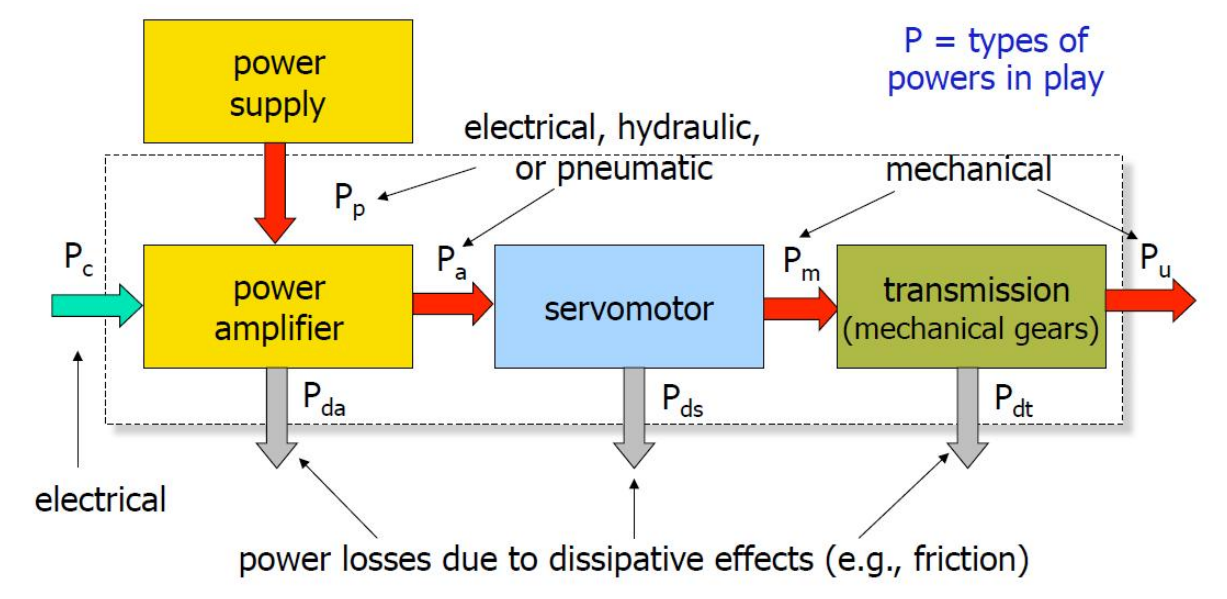
\includegraphics[width=.78\linewidth]{01-actuation-system.png}
\caption{动力源、功率放大器、执行元件和传动装置。取自《Actuators》PDF 第24页。}
\label{fig:actuation-system}
\end{figure}

\begin{table}[htbp]
\centering\small
\begin{tabularx}{\linewidth}{@{}l X X@{}}
\toprule
方式 & 工作特点 & 选型与应用 \\
\midrule
电动 & 电机由电压、电流驱动，便于与编码器组成精确伺服。电机通电保持负载时会产生铜损。 & 常见于工业机器人关节。校核发热、供电和制动保持需求。 \\
液压 & 由压力液体驱动液压缸或马达，可在低速下输出很大的力或转矩。 & 适合重载。需油源与阀组，并考虑泄漏、维护和系统体积。 \\
气动 & 压缩空气驱动，结构可较简单，气体压缩性使系统具有柔顺性。 & 适合开合与简单往复，如夹爪。负载变化时，精确轨迹控制较难。 \\
\bottomrule
\end{tabularx}
\end{table}

\textbf{机器人关节的典型要求}包括高功率重量比、低惯量、启停与换向能力、宽速域和低速平稳性。定位准确度看实际位置偏离目标的程度，重复定位精度看相同命令下位置的离散程度。

\FloatBarrier
\section{永磁直流电机的机电模型}

\subsection{洛伦兹力与换向}

均匀磁场中，一段方向沿电流的导线 $\boldsymbol{\ell}$ 受到 $\boldsymbol{F}=i_a\boldsymbol{\ell}\times\boldsymbol{B}$。矩形线圈两侧的电流方向相反，磁场力也相反，形成力偶。用 $d$ 表示每侧距转轴的距离，按图\ref{fig:actuator-commutation}的角度约定，单匝有效力臂为 $d\cos\theta$，转矩大小随角度按 $2d|F\cos\theta|$ 变化。为了连续转动，有刷直流电机利用电刷与换向器在转子转过相应位置时改变线圈电流方向，使转矩保持同向。多绕组错相布置可减小转矩脉动。

\begin{figure}[htbp]
\centering
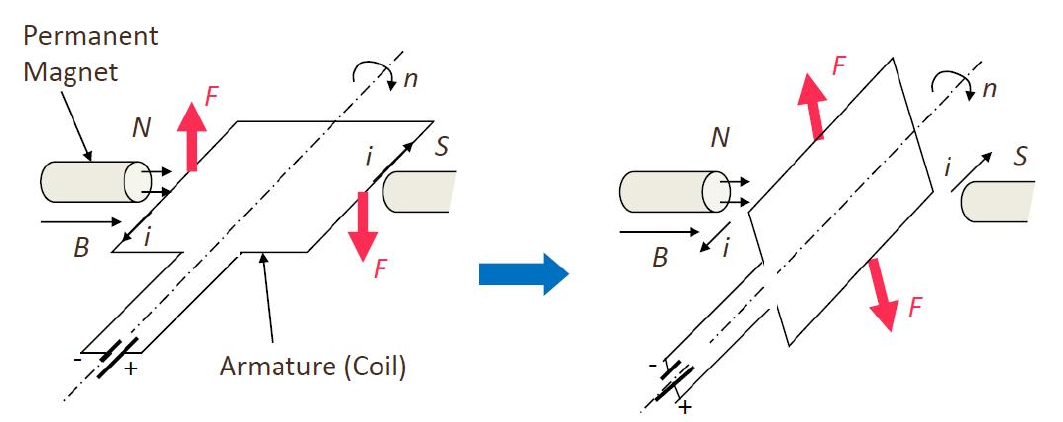
\includegraphics[width=.79\linewidth]{01-dc-motor-commutation.png}
\caption{线圈两侧的磁场力及其力臂。取自《Actuators》PDF 第7页的示意图。}
\label{fig:actuator-commutation}
\end{figure}

\subsection{电路、转矩与机械运动}
\label{sec:actuator-equations}

设电枢电压 $u$、电流 $i_a$、电阻 $R$、电感 $L$，电机角速度 $\omega_m$，电磁转矩 $\tau_e$。取电压、电流和转矩的正方向一致，并把折算到电机轴的外部负载转矩 $\tau_L$ 定为正转时的阻转矩。线性模型为
\begin{align*}
 u &= Ri_a+L\frac{\mathrm di_a}{\mathrm dt}+e_b,
 & e_b&=K_e\omega_m,\\
 \tau_e&=K_t i_a,
 &J\frac{\mathrm d\omega_m}{\mathrm dt}+B\omega_m&=\tau_e-\tau_L .
\end{align*}
这里 $J$ 是按所选轴折算的惯量，$B$ 为黏性阻尼系数。若 $J$ 已含负载惯量，$\tau_L$ 只计其余阻转矩。反电动势由转子旋转产生，在正向电动工况中压低同电压下的电流。乘以电流可写成
\[
ui_a=Ri_a^2+\frac{\mathrm d}{\mathrm dt}\left(\frac12 Li_a^2\right)+e_bi_a.
\]
理想机电转换满足 $e_bi_a=\tau_e\omega_m$，故在 $K_t$ 用 $\mathrm{N\,m/A}$、$K_e$ 用 $\mathrm{V\,s/rad}$ 时，两者数值相等。若手册给出 $\mathrm{rpm/V}$ 的速度常数 $K_v$，转为上述单位应取 $K_e=60/(2\pi K_v)$。零初值下令 $\tau_L=0$，消去电流，可得电压到角速度的模型
\[
\frac{\Omega_m(s)}{U(s)}=\frac{K_t}{(Ls+R)(Js+B)+K_tK_e}.
\]
固定转子时，电流的一阶时间常数为 $L/R$。忽略电枢电感时，角速度的一阶时间常数为 $J/(B+K_tK_e/R)$，角位置模型再乘 $1/s$。

\nt{\textbf{建模条件}　稳态电流允许略去 $L\,\mathrm di_a/\mathrm dt$，瞬态电流响应要保留电感。手册中绕组温度变化会改变 $R$，精细选型需使用相应温度下的工作参数。}

\FloatBarrier
\section{矩速曲线与参数表}

在恒定端电压 $U$ 下，取稳态并忽略机械损耗，$\tau=\tau_e$，从 $U=R\tau/K_t+K_e\omega$ 得
\[
\boxed{\omega=\frac{U}{K_e}-\frac{R}{K_e K_t}\tau},\qquad
\omega_0=\frac{U}{K_e},\qquad \tau_s=K_t\frac{U}{R}.
\]
$\omega_0$ 是理想空载转速，$\tau_s$ 是理想堵转转矩。在实际电机中，空载仍需小电流克服摩擦等损耗，实际空载转速略低于上述理想值。在这个模型和端电压下，轴机械功率为
\[
P_{\mathrm{out}}=\tau\omega=\omega_0\tau\left(1-\frac{\tau}{\tau_s}\right),\qquad
P_{\max}=\frac{\tau_s\omega_0}{4}
\quad\text{当 }\tau=\frac{\tau_s}{2},\ \omega=\frac{\omega_0}{2}.
\]
堵转和理想空载的轴输出功率都为零。堵转仍可能伴随很大的电流和温升；在此理想模型中，最大机械功率点的效率为 $1/2$，等于该点反电动势与端电压的比值。

\begin{figure}[htbp]
\centering
\begin{tikzpicture}
\begin{axis}[
  width=.74\linewidth,height=4.45cm,xmin=0,xmax=1.08,ymin=0,ymax=1.19,
  axis lines=left, xlabel={$\tau/\tau_s$}, ylabel={归一化值},
  xtick={0,.5,1},xticklabels={$0$,$1/2$,$1$},
  ytick={0,.5,1},yticklabels={$0$,$1/2$,$1$},
  legend style={at={(.5,1.03)},anchor=south,legend columns=2,draw=none,font=\small}]
\addplot[myb,very thick,domain=0:1] {1-x};
\addlegendentry{$\omega/\omega_0$}
\addplot[myr,very thick,dashed,domain=0:1,samples=50] {4*x*(1-x)};
\addlegendentry{$P_{\mathrm{out}}/P_{\max}$}
\draw[densely dotted,gray] (axis cs:.5,0)--(axis cs:.5,1);
\end{axis}
\end{tikzpicture}
\caption{恒压条件下的理想矩速曲线和机械功率曲线。依据《Actuators》PDF 第14页重绘。}
\label{fig:actuator-torque-speed}
\end{figure}

\textbf{读电机参数表时先认运行条件。}额定功率对应指定工况。连续转矩受温升限制，峰值转矩还受驱动限流和持续时间限制。最大机械功率点、最大效率点与额定点各有定义。电机常数 $K_m=K_t/\sqrt R$，同转矩下可用 $P_{\mathrm{Cu}}=\tau_e^2/K_m^2$ 比较铜损。

\ex{由端电压求工作点}{设 $U=24\,\mathrm V$、$R=2\,\Omega$、$K_t=0.10\,\mathrm{N\,m/A}$、$K_e=0.10\,\mathrm{V\,s/rad}$。忽略机械损耗，稳态负载转矩为 $0.30\,\mathrm{N\,m}$。求电流、转速、轴功率，并检验功率平衡。}

\textbf{解}　先按转矩算电流，再按电压平衡求转速。
\[
i_a=\frac{0.30}{0.10}=3.0\,\mathrm A,\qquad
\omega=\frac{24-2\times3}{0.10}=180\,\mathrm{rad/s}.
\]
机械输出为 $0.30\times180=54\,\mathrm W$；电输入 $24\times3=72\,\mathrm W$，铜损 $3^2\times2=18\,\mathrm W$。两项相加等于输入功率。由曲线截距公式得 $\tau_s=1.2\,\mathrm{N\,m}$、$\omega_0=240\,\mathrm{rad/s}$，理想最大轴功率为 $72\,\mathrm W$。

\FloatBarrier
\section{传动与关节负载折算}
\label{sec:actuator-transmission}

\textbf{减速比与传动效率}　取减速比 $N=\omega_m/\omega_j>1$，电机向负载供能时，若传动效率为 $\eta$，有
\[
\boxed{\omega_j=\omega_m/N,\qquad \tau_j=\eta N\tau_m},\qquad
P_j=\eta P_m .
\]
下标 $m,j$ 分别为传动输入电机侧和输出关节侧。机构反转时须另计旋向。

由齿轮、同步带或其他机构实现减速增扭；丝杠可将旋转变为平移。若丝杠导程 $p$ 指一转的轴向位移，则前向驱动时 $v=p\omega/(2\pi)$；以效率 $\eta$ 和功率平衡计算推力 $F=2\pi\eta\tau/p$。传动还能把电机布置在靠近基座处，以减轻运动部件，但要考虑间隙、摩擦和柔性。

\textbf{惯量折算由动能决定。}忽略传动件自身惯量，负载惯量 $J_j$ 的动能为
\[
\frac12 J_j\omega_j^2=\frac12 \frac{J_j}{N^2}\omega_m^2.
\]
因此 $J_j$ 折算至电机轴为 $J_j/N^2$；反过来，电机转子惯量 $J_m$ 折算至关节为 $N^2J_m$。前向传动的效率用于按功率折算转矩，动能等效本身由速度比决定。较高减速比可减小电机轴所见负载惯量，同时增大关节所见转子惯量，并提高相同关节速度所要求的电机转速。

电机选型时，可据力臂和加速度求关节转矩，再按传动关系映射到电机。比较具体工作点的可用转矩和转速；有重复工作周期且铜损占主导时，用 $\tau_{\mathrm{rms}}=\sqrt{\sum_k\tau_k^2\Delta t_k/\sum_k\Delta t_k}$ 初估发热，另行校核峰值、散热和实际矩速包络。

\ex{减速器与电机轴的需求}{关节负载惯量 $J_j=0.18\,\mathrm{kg\,m^2}$，运动时有恒定阻转矩 $5.0\,\mathrm{N\,m}$。关节从静止以恒加速度在 $0.20\,\mathrm s$ 内达到 $1.20\,\mathrm{rad/s}$。传动比 $N=12$、前向效率 $\eta=0.90$，电机转子惯量 $J_m=0.002\,\mathrm{kg\,m^2}$。忽略其他惯量和损耗，求加速阶段所需的电磁转矩和阶段末转速。}

\textbf{解}　关节角加速度为 $6.0\,\mathrm{rad/s^2}$，所需输出转矩为 $5.0+0.18\times6.0=6.08\,\mathrm{N\,m}$。电机轴传入减速器的转矩为 $6.08/(0.90\times12)=0.563\,\mathrm{N\,m}$，电机转子另需 $J_mN\alpha_j=0.144\,\mathrm{N\,m}$，故
\[
\tau_e\approx0.707\,\mathrm{N\,m},\qquad \omega_m=12\times1.20=14.4\,\mathrm{rad/s}.
\]
恒速后，因角加速度为零，电磁转矩降为 $5.0/(0.90\times12)\approx0.463\,\mathrm{N\,m}$。选型时需校核 $14.4\,\mathrm{rad/s}$ 附近约 $0.707\,\mathrm{N\,m}$ 的短时能力及约 $0.463\,\mathrm{N\,m}$ 的恒速负载条件。

\section{驱动器如何进入控制回路}

机器人控制从任务规划、轨迹规划到关节伺服逐层展开。直接控制层用模型和反馈生成驱动命令。位置闭环根据 $q_d-q$ 跟踪目标，转矩闭环根据 $\tau_d-\tau$ 调节关节输出，外层还可根据位置、速度或接触力给定目标转矩。相关控制律见第5章。

\begin{focusbox}{考前自测}
\begin{enumerate}[nosep]
\item 给定理想电机参数 $U,R,K_t,K_e$，如何标出空载点、堵转点、最大机械功率点？堵转电流是多少？
\item 减速比翻倍、关节转速保持不变时，两端所见惯量和电机转速如何变化？
\item 重载低速、精密连续轨迹、简单开合各可考虑哪类驱动？
\end{enumerate}
\textbf{核对}　$\omega_0=U/K_e$，$\tau_s=K_tU/R$，最大功率点为两个截距的一半，$i_s=U/R$。减速比翻倍使电机转速翻倍，电机侧负载惯量变为 $1/4$，关节侧电机惯量变为四倍。三种任务可分别考虑液压伺服、电伺服和气缸，并结合具体负载和环境核实。
\end{focusbox}

{\small 本章依据《Actuators》PDF 第4至17、19至20、24至26、29、32、34至39、45至47页整理。惯量匹配和周期热校核用于理解关节选型，拓展资料见《人形机器人关节电机选型方法论》。}

\chapter{机器人传感技术}
\label{chap:robot-sensing}

\begin{focusbox}{本章复习路线}
看到一个传感器，先说清\textbf{测什么、如何转换、读数代表什么}。计算题优先掌握编码器的分辨角、辨向与测速，以及力和力矩的参考点变换、超声脉冲测距。简答题重点比较绝对式与增量式编码器、关节式与腕部六维力传感器，并能解释接近觉、触觉和视觉各自提供的信息。
\end{focusbox}

\section{内部状态与外部环境}

按被测对象划分，\textbf{内部传感器}提供本体状态，如关节位置、速度、加速度与内部载荷。\textbf{外部传感器}获取环境、目标或接触信息，如障碍物距离、表面压力分布与物体图像。安装在机器人上的相机仍可感知外部目标；腕部力传感器用于读出环境接触载荷时提供外部交互信息。判断分类时用被测信息和用途来说明理由。

位置反馈可采用电阻式、电容式、电感式、光电式、霍尔元件或磁栅等方法。均匀电位器在高输入阻抗读出条件下近似为分压器。若滑动端位移为 $x$、有效行程为 $l$、激励电压为 $U_e$，并以滑动起点为低电位端，则 $U_o\simeq U_e x/l$。旋转电位器可把 $x/l$ 换成角行程比例。传感器选型同时检查量程、分辨率、定位误差、重复性、动态响应和工作环境。

\section{旋转编码器}
\label{sec:rotary-encoders}

\subsection{绝对式读码与增量式计数}

\dfn{绝对式编码器}{输入轴转到某个角区时，多条码道同时给出该角区的码字。若 $n$ 位码覆盖一整圈并均匀编码，单圈位置数为 $2^n$，最小分辨角为 $\Delta\theta=360^\circ/2^n$。单圈绝对码上电可读出圈内位置，圈数需要多圈能力或其他信息。}

光学式绝对编码器通过检测各码道的透光与遮光状态读位，也可用接触型码盘帮助理解编码结构。自然二进制从 $0111$ 切到 $1000$ 时多位同时变化，边界处各码道的读出时刻若有偏差，可能产生跳码。格雷码的相邻位置只变一位，可减少这种多位跳变错误。编码读取后需按实际码制译码。对反射格雷码，从最高位向最低位用 $b_{n-1}=g_{n-1}$，$b_k=b_{k+1}\oplus g_k$ 恢复自然二进制。

\begin{figure}[htbp]
\centering
\begin{minipage}[b]{.542\linewidth}
\centering
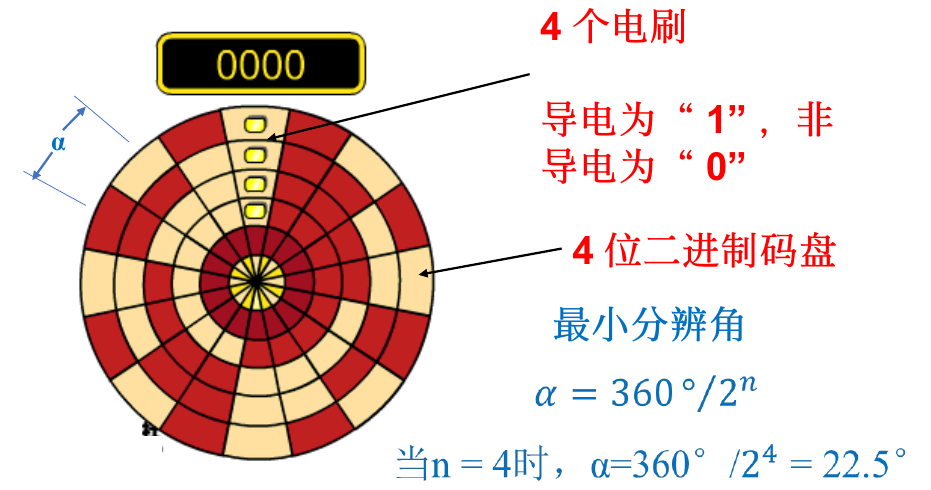
\includegraphics[width=\linewidth]{02-absolute-code-disc.png}\\[-.1em]
{\small (a) 接触式四位绝对码盘}
\end{minipage}\hfill
\begin{minipage}[b]{.425\linewidth}
\centering
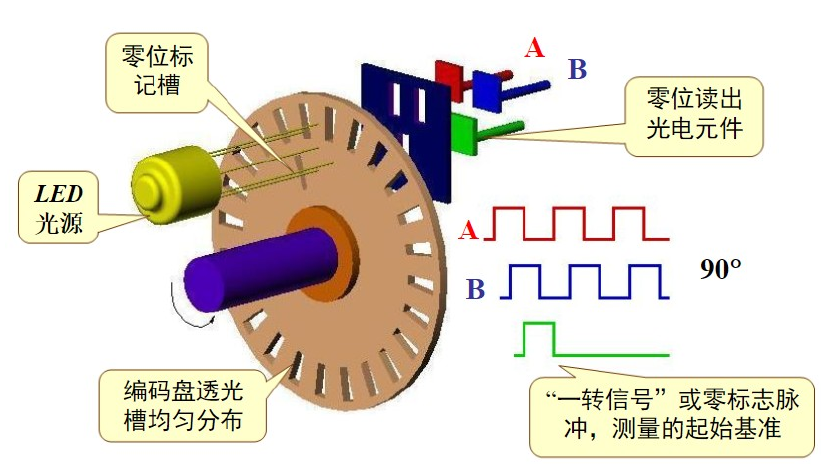
\includegraphics[width=\linewidth]{02-incremental-encoder.png}\\[-.1em]
{\small (b) 增量式光电编码器}
\end{minipage}
\caption{绝对式码盘的多码道与增量式编码器的 A/B/Z 信号。取自《第2章：机器人传感技术》第12、15张。}
\label{fig:encoder-principle}
\end{figure}

增量式编码器的透光条纹产生周期脉冲。A、B 相相差 $90^\circ$ 电相位，讲义约定 A 超前 B 时为正转，反过来为反转。该相位差是单个信号周期的四分之一。Z 相通常每转一脉冲，可在回零流程中提供参考标志。正交解码可数 A 相单边沿（$m=1$）、A 相双边沿（$m=2$）或 A、B 相全部边沿（$m=4$）。约定 $P$ 为 A 相每转的完整周期数，在同一解码方式下
\[
C=mP,\qquad \Delta\theta=\frac{2\pi}{C},\qquad
\theta-\theta_{\mathrm{ref}}=n_c\frac{2\pi}{C},\qquad
\overline\omega=\frac{2\pi\Delta n_c}{C\Delta t}.
\]
其中 $C$ 为实际每转计数，$n_c$ 是自参考位置累加的带符号计数。若手册已直接给出每转计数，应以该计数为 $C$。停电后若累加计数丢失，需重建参考位置。用固定时间窗测速时，低速可能只读到少数计数，可采用边沿间隔估计或在允许延迟时加长时间窗。

\nt{\textbf{分辨率、精度与安装位置}　解码倍频缩小名义分辨角。称为角度精度时还要考虑码盘偏心、相位误差和机械间隙。电机侧编码器经减速比换算得到理想关节读数；关节输出端的间隙、弹性变形需另行建模或测量。}

\ex{增量式编码器的转角和转速}{电机编码器 A 相每转 $1024$ 个完整周期，A、B 相所有边沿均计数。$40\,\mathrm{ms}$ 内计数净增 $128$，采用 A 超前 B 为正向的约定。求电机角增量与平均转速。若电机经同向理想 $8{:}1$ 减速器带动关节，再求关节侧数值。}

\textbf{解}　四倍计数时 $C=4096$，所以电机轴一计数对应 $360^\circ/4096=0.08789^\circ$。窗口内角增量及平均转速为
\[
\Delta\theta_m=\frac{128}{4096}\,360^\circ=11.25^\circ,
\qquad n_m=\frac{128}{4096\times0.040}\,60=46.875\,\mathrm{rpm}.
\]
关节角增量为 $1.40625^\circ$，平均转速为 $5.859375\,\mathrm{rpm}$。角增量和速度都带正号。若换用 A 相单边沿计数，同一实际转角只产生 $32$ 个计数，重新用 $C=1024$ 换算也得到同样的角增量。

\ex{绝对式编码器的格雷码译码}{四位单圈绝对式编码器采用反射格雷码，当前输出 $1000$，设自然二进制零码对应 $0^\circ$，正向每级角度按均匀格点换算。求角度标称值。}

\textbf{解}　逐位异或有 $b_3=1$、$b_2=1\oplus0=1$、$b_1=b_0=1$，得到自然二进制 $1111=15$。每级分辨角 $360^\circ/16=22.5^\circ$，标称位置为 $15\times22.5^\circ=337.5^\circ$。原码 $1000$ 与下一圈零码 $0000$ 也只相差一位。

\FloatBarrier
\section{力、力矩与六维力传感}
\label{sec:robot-force-sensing}

\subsection{机械载荷如何变为电信号}

关节式力矩传感器通常测单个关节轴的转矩。载荷使弹性元件发生扭转，应变片把应变变为相对电阻变化 $\Delta R/R=K_g\varepsilon$，再经激励电桥读出电压。测量链可写成
\[
\text{关节转矩}\longrightarrow\text{弹性变形}\longrightarrow
\varepsilon\longrightarrow\Delta R\longrightarrow U_o .
\]
在线性区，若等臂单臂电桥的受拉应变片是输出支路的下臂，输出取该支路中点电压减参考支路中点电压，则 $U_o\simeq U_e K_g\varepsilon/4$。接法决定输出极性，实际标定把电压映射回转矩。

腕部六维力传感器通常安装在机械臂腕部与末端工具之间，提供三个力分量和关于指定参考点的三个力矩分量。选择不同弹性结构与应变片位置，使各加载方向产生可区分的应变组合。若若干通道的读数为 $\mathbf y$，定义力旋量 $\boldsymbol w=[F_x,F_y,F_z,M_x,M_y,M_z]^{\mathsf T}$。线性标定可写为
\[
\mathbf y=\mathbf A\boldsymbol w+\mathbf b .
\]
$\mathbf b$ 为零点偏置。方阵 $\mathbf A$ 可逆时，用 $\mathbf A^{-1}(\mathbf y-\mathbf b)$ 恢复六个分量；对多通道满列秩的情形可用最小二乘标定与解算。标定矩阵的非对角耦合反映单通道可能同时响应多个力或力矩分量。

\begin{figure}[htbp]
\centering
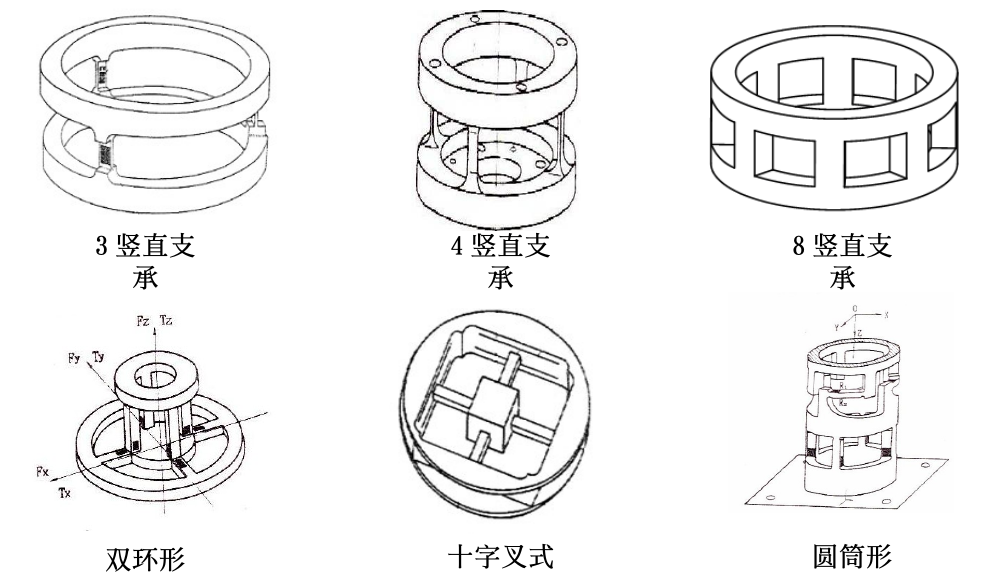
\includegraphics[width=.73\linewidth]{02-six-axis-structures.png}
\caption{腕部六维力传感器的几种弹性体结构。取自《第2章：机器人传感技术》第20张。}
\label{fig:six-axis-structures}
\end{figure}

\subsection{力矩的参考点与无传感器估计}

同一个力用同一坐标轴表示时，改变参考点只改变对应力矩。若 $\boldsymbol r_{OC}$ 从新参考点 $O$ 指向原参考点 $C$，则
\[
\boldsymbol F_O=\boldsymbol F_C,\qquad
\boldsymbol M_O=\boldsymbol M_C+\boldsymbol r_{OC}\times\boldsymbol F_C .
\]
若坐标轴同时改变，还应把两个三维向量旋转到同一坐标系后再做叉乘。

也可由电机电流 $\tau_e=K_t i_a$ 估计电磁转矩，经传动折算并扣除机器人惯性、重力、摩擦等模型项后，估计外力在关节上的等效转矩。以 $\boldsymbol w_{\mathrm{ext}}$ 表示环境作用于机器人、与雅可比 $\mathbf J$ 用同一坐标系、参考点和力/速度分量顺序表示的力旋量。由虚功关系
\[
\boldsymbol\tau_{\mathrm{ext}}^{\mathsf T}\delta\boldsymbol q
=\boldsymbol w_{\mathrm{ext}}^{\mathsf T}\mathbf J\delta\boldsymbol q
\quad\Longrightarrow\quad
\boldsymbol\tau_{\mathrm{ext}}=\mathbf J^{\mathsf T}\boldsymbol w_{\mathrm{ext}} .
\]
单末端接触假设下，能否由关节残差唯一估计六维力旋量取决于 $\mathbf J$ 的秩。摩擦误差、模型误差、未知接触位置与奇异位形都会影响估计。

\Needspace{12\baselineskip}
\ex{腕部测力中的参考点}{传感器与接触点的坐标轴平行。从腕部传感器原点 $O$ 指向接触点 $C$ 的位置向量为 $(0.06,0.02,0)^{\mathsf T}\,\mathrm m$。接触点有力 $\boldsymbol F_C=(0,0,20)^{\mathsf T}\,\mathrm N$ 和力矩 $\boldsymbol M_C=(0,0,0.10)^{\mathsf T}\,\mathrm{N\,m}$。求关于 $O$ 的六维载荷。}

\textbf{解}　力分量保持原值，力作用点平移造成附加力矩
\[
\boldsymbol r_{OC}\times\boldsymbol F_C
=\begin{bmatrix}0.02\times20\\-0.06\times20\\0\end{bmatrix}
=\begin{bmatrix}0.40\\-1.20\\0\end{bmatrix}\,\mathrm{N\,m}.
\]
故关于腕部原点的力矩为 $(0.40,-1.20,0.10)^{\mathsf T}\,\mathrm{N\,m}$，与力 $(0,0,20)^{\mathsf T}\,\mathrm N$ 组成六维载荷。若已知腕部读数并要换算到接触点，则减去上述附加力矩。

\FloatBarrier
\section{接近觉、测距与触觉}

\begin{table}[htbp]
\centering\small
\begin{tabularx}{\linewidth}{@{}p{2.2cm} X X@{}}
\toprule
方式 & 转换链 & 使用条件 \\
\midrule
电涡流 & 线圈交变磁场在导电目标中激起涡流，涡流反作用改变线圈阻抗。 & 适合导电目标的近距离检测，读数也随材料与几何条件变化。 \\
超声波 & 发射脉冲，接收回波；已知声速 $c$ 和往返时差 $\Delta t$，得 $d=c\Delta t/2$。 & 声速随介质和温度变化；发射振铃造成近场盲区，倾斜或吸声面可能回波弱。 \\
主动红外 & 发射调制红外光，接收目标反射后解调，可判断物体接近。 & 与目标表面反射率、入射角及背景光有关。反射强度式需标定，测距型还可用三角或飞行时间原理。 \\
\bottomrule
\end{tabularx}
\end{table}

\textbf{触觉信息有层次。}开关式触觉只提供接触与否；分布式接触传感器还能定位接触区域；压觉或力觉给出接触强弱；滑觉用来识别物体与夹爪的相对滑动，便于调节握持力。压阻阵列的行、列电极交叉处构成触元，受压使局部电阻改变，逐行列扫描可恢复压力分布。性能受触元密度、灵敏度、柔顺性和耐用性共同约束。探测到压强 $p_k$ 的触元有效面积为 $A_k$ 时，各触元法向力近似为 $p_kA_k$；在接触面近似平坦且压力方向平行时可由 $\sum_k p_kA_k$ 估算法向总力。

\begin{figure}[htbp]
\centering
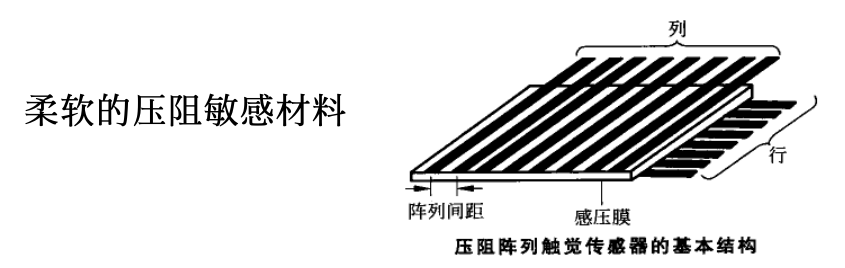
\includegraphics[width=.71\linewidth]{02-tactile-array.png}
\caption{压阻阵列的行列电极与触元结构。取自《第2章：机器人传感技术》第30张。}
\label{fig:tactile-array}
\end{figure}

\ex{超声飞行时间测距}{一只同处发射与接收的超声测距模块，在已知空气声速 $c=343\,\mathrm{m/s}$ 的条件下测得脉冲往返时间为 $8.0\,\mathrm{ms}$。忽略内部延迟，求单程障碍物距离。}

\textbf{解}　$\Delta t$ 覆盖从传感器到障碍物再返回的路程，故 $d=343\times0.0080/2\approx1.37\,\mathrm m$。若电路有固定延迟，先从实测时差中扣除该延迟再代入飞行时间公式。

\FloatBarrier
\Needspace{8\baselineskip}
\section{视觉传感器与成像元件}

视觉系统通常由照明、镜头、相机、图像处理器和算法组成。先用照明把目标特征和背景分开，再由镜头成像，传感器完成光电转换和场景离散化，图像算法提取控制需要的目标信息。检测轮廓时可考虑背光突出边界，观察表面细节时则可用适合反射特性的照明。

\begin{itemize}
\item \textbf{焦距与视场}　在传感器尺寸和成像模型固定时，较短焦距给出较大视场角。理想直线投影的水平视场角可近似为 $2\arctan(w/(2f))$，其中 $w$ 为有效传感器宽度，$f$ 为焦距。镜头分类应结合画幅和投影方式，鱼眼镜头的投影关系要单独考虑。
\item \textbf{光圈与景深}　光圈数 $N_f=f/D$，$D$ 为入瞳直径。光圈数增大时开口相对缩小；在相同焦距、对焦距离和弥散标准下，通常进光减少而景深增大。缩得过小时，衍射也会影响清晰度。
\item \textbf{CCD 与 CMOS}　两者都利用光生电荷感光。典型 CCD 逐级转移电荷，汇至少数输出节点转换并读出；典型 CMOS 在像素有电荷电压转换能力，可借助行列寻址与并行通道读出，便于实现高集成和低功耗。噪声、帧率及动态范围需按器件规格与曝光方式判断。
\end{itemize}

\begin{focusbox}{考前自测}
\begin{enumerate}
\item 已知 $12$ 位单圈绝对编码器和 $1024$ 周期/转的增量式编码器（四倍计数），二者名义分辨角有何关系？各自的读数如何对应角位置？
\item 只测腕部法向力大小时，能否区分同方向等大小但作用点不同的两个力？六维传感器多提供了什么信息？
\item 对金属近接检测、移动机器人障碍物测距、夹持滑动判断，各选哪类传感器？
\end{enumerate}
\textbf{核对}　两者均为 $360^\circ/4096$；绝对式直接译码得到圈内位置，增量式由参考点和带符号计数求位置。法向力一样时需利用关于同一参考点的力矩分量判断力线偏移。三项任务分别可用电涡流探头、超声脉冲测距模块与滑觉传感器。
\end{focusbox}

{\small 本章依据《第2章：机器人传感技术》第3至4、7至15、17至30、33至41张整理。格雷码、四倍计数、分辨率与精度的辨析也参考《编码器核心技术深度解析与应用趋势》第7、9、13页。}

\chapter{图像形成}
\label{chap:rii-image-formation}

\begin{focusbox}{本章复习路线}
从检测任务出发，先定照明、视野与像素分辨率，再把空间点沿“世界坐标 $\to$ 相机坐标 $\to$ 图像坐标 $\to$ 像素坐标”的顺序投影。做尺寸测量时，按标定结果把提取到的像点还原到已知测量面。\textbf{优先练习}相机与镜头选型计算、内外参投影、畸变与标定流程、平面尺寸及圆拟合。
\end{focusbox}

本章对应《第3章：图像形成》讲义。系统组成与选型见 PDF 第10--85页，重点例题见第50--54、75--81页。成像与标定见第103--123页，视觉测量见第124--135页。讲义中的行业案例用于理解任务类型。

\section{机器视觉系统与选型}

典型流程为\textbf{触发采集 $\to$ 照明与成像 $\to$ 图像传输 $\to$ 分析与输出}。触发传感器确定拍摄时机，镜头把场景投到感光靶面，相机完成光电转换与数字化，处理器给出计数、定位、尺寸或缺陷判定。搭建系统时先明确\textbf{想看见哪种差异}，再确定采集参数。

\subsection{照明方式与应用}

\begin{table}[htbp]
\centering\small
\begin{tabularx}{\linewidth}{@{}p{2.5cm} X X@{}}
\toprule
方式 & 成像机制 & 典型任务 \\
\midrule
背光 & 光源位于工件后方，形成高对比度的剪影 & 外轮廓、孔径、液位与遮挡检测 \\
同轴光 & 光经分光元件沿相机轴线照向工件，平整区域的反光进入镜头 & 平整反光表面上的标记或缺陷 \\
暗场光 & 低角度光照射，平面镜面反射绕开镜头，划痕散射入镜 & 低对比度划痕、凹坑及边缘 \\
明场光 & 正面照明，让背景较亮，异常区域产生明暗差异 & 普通表面纹理、字符、灰度对比检测 \\
弥散穹顶 & 从多方向均匀照射，减弱高光与阴影 & 曲面、光泽表面与不规则工件 \\
结构光 & 投射已知光条、点阵或编码图案，利用变形和几何关系测深 & 高度差、轮廓与三维形貌 \\
\bottomrule
\end{tabularx}
\end{table}

光色也会改变灰度对比。以单色相机为例，若表面主要反射红光，红光照明可使红色区域变亮；使用其反射率较低的照明波段可使该区域变暗。实际选择还要看相机的光谱响应和其他区域的反射率。

\subsection{工业相机、视野与曝光}

相机选型先判断单帧的空间覆盖要求。\textbf{面阵}直接输出二维帧，适合固定区域拍照。\textbf{线阵}每次采集一行，依靠物体与相机的相对运动拼成二维图，适合卷材等连续物料。若输送速度为 $v$、沿运动方向所需的物方采样间距为 $q$，则线阵的行频至少为 $v/q$，速度变化时通常用编码器同步。黑白相机便于做单通道灰度测量，依靠颜色区分的任务可用彩色相机与合适的光源。CCD 典型地逐级转移并读出电荷，CMOS 成像单元通常可在芯片内完成放大及分列读出。具体快门方式应看型号。

\dfn{像元、靶面与物方采样间距}{设相机分辨率为 $N_x\times N_y$，每个像元的物理尺寸为 $d_x\times d_y$，则靶面宽高为 $S_x=N_xd_x$、$S_y=N_yd_y$，对角长为 $\sqrt{S_x^2+S_y^2}$。在平行于靶面且可用均匀尺度的测量平面，视野宽高为 $W_x\times W_y$ 时，每像素的物方尺寸为
\[
q_x=\frac{W_x}{N_x},\qquad q_y=\frac{W_y}{N_y}.
\]
若尺寸为 $a$ 的最小特征必须跨越至少 $n$ 个像素，则对应方向 $q\le a/n$，所需像素数 $N\ge\lceil Wn/a\rceil$。位深为 $b$ 的单通道理想量化级数为 $2^b$。}

\textbf{全局曝光}使各行的感光时段一致。\textbf{卷帘曝光}逐行开始或结束，快速运动会使同一帧里的各行记录不同位置，从而产生几何变形。两种快门的单次曝光都可能产生拖影。在物平面内物体以速度 $v$ 匀速横移，若该方向的物方采样间距为 $q$，希望曝光内的拖影不超过 $m$ 个像素，则
\[
t_{\mathrm{exp}}\le \frac{mq}{|v|}.
\]
帧率决定多久取得下一帧，曝光时间决定单帧内积分多久。实际缩短曝光时需同时检查照明、噪声和相机吞吐量。

\begin{figure}[htbp]
\centering
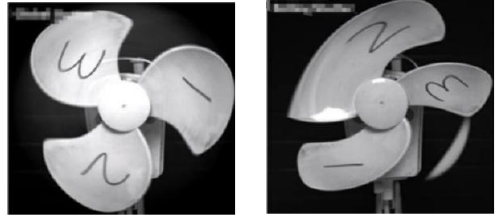
\includegraphics[width=0.46\linewidth]{03-shutters.png}
\caption{转动叶片的全局曝光（左）和卷帘曝光（右）。裁自《第3章：图像形成》PDF 第48页。}
\label{fig:rii-shutters}
\end{figure}

\subsection{镜头、工作距离与景深}

薄透镜模型用物距 $Z$、像距 $s'$、焦距 $f$ 描述合焦条件。沿同一方向设物方视野为 $W$、靶面宽度为 $S$，有
\[
\frac1f=\frac1Z+\frac1{s'},\qquad
|\beta|=\frac{S}{W}=\frac{s'}{Z},\qquad
f=\frac{ZS}{W+S}.
\]
当 $Z\gg f$ 时可令 $s'\approx f$。若题目以工作距离 $\mathrm{WD}$ 近似从镜头主平面量得的 $Z$，则使用讲义中的选型估算 $W\approx \mathrm{WD}\,S/f$。给同一个方向的靶面尺寸 $S$，远距近似下视场角为 $2\arctan[S/(2f)]$。\textbf{固定工作距离和靶面时，焦距越长，视野越小。}

光圈数 $F=f/D$，其中 $D$ 为有效孔径。其余条件相同，缩小光圈（增大 $F$）通常增大景深、减少通光量，成像面照度近似与 $1/F^2$ 成正比。景深是满足清晰度要求的物距范围。尺寸测量若有小幅工件高度变化，可选\textbf{物方远心镜头}使倍率在有效工作范围内对深度变化较不敏感。选镜头还应核对像圈覆盖、接口、畸变和分辨能力。

\Needspace{5\baselineskip}
\ex{从字符笔画估算分辨率、焦距与曝光}{
检测区为 $110\,\mathrm{mm}\times27\,\mathrm{mm}$，需留位置余量，设计视野为 $160\,\mathrm{mm}\times120\,\mathrm{mm}$。最窄笔画宽 $0.5\,\mathrm{mm}$，要求跨过至少 10 像素。靶面宽 $6.4\,\mathrm{mm}$，工作距离约 $400\,\mathrm{mm}$。若工件沿图像水平方向以 $200\,\mathrm{mm/s}$ 匀速移动，按设计采样间距估算允许 1 像素拖影时的曝光时间。
\begin{enumerate}
\item 采样间距上限为 $q=0.5/10=0.05\,\mathrm{mm/pixel}$。取该间距设计，得 $N_x\ge160/0.05=3200$、$N_y\ge120/0.05=2400$，最低约 $7.68$ 百万像素，宽高各自也要达标。
\item 代入远距估算得 $f\approx400\times6.4/160=16\,\mathrm{mm}$。若按理想薄透镜精算，则 $f=400\times6.4/(160+6.4)\approx15.38\,\mathrm{mm}$。实际选接近规格后要复核视野及合焦范围。
\item $t_{\mathrm{exp}}\le0.05/200=2.5\times10^{-4}\,\mathrm{s}=0.25\,\mathrm{ms}$。采用更密的采样时，同一像素拖影限制对应更短的曝光。
\end{enumerate}
}

\nt{“每个特征跨 10 像素”是本例要求。题目给出像素覆盖或定位精度时应按其条件计算，物方采样间距也不能直接作为最终测量误差。镜头与标定误差、噪声、机械振动及边缘定位方法都会影响测量。}

\section{针孔成像与相机标定}

\subsection{四个坐标系与内外参}

\noindent\keypoint{复习重点：外参先把世界坐标变到相机坐标，然后除以相机深度，最后应用内参得到像素。}

设世界点 $\mathbf P_w=(X_w,Y_w,Z_w)^\mathsf T$，使用列向量且规定外参方向为世界到相机。相机坐标为 $\mathbf P_c=R\mathbf P_w+\mathbf t$，其中 $R^\mathsf TR=I$、$\det R=1$。相机中心在世界系中的坐标为 $\mathbf C_w=-R^\mathsf T\mathbf t$，即令 $\mathbf P_c=\mathbf 0$ 所得的位置。

\begin{figure}[htbp]
\centering
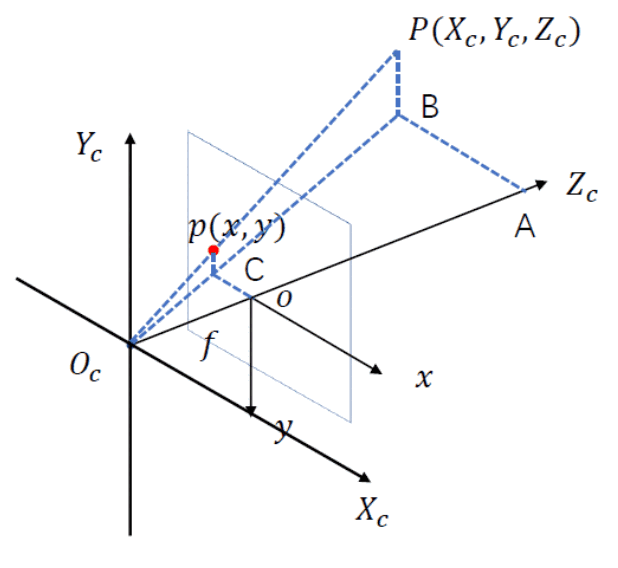
\includegraphics[width=0.51\linewidth]{03-perspective.png}
\caption{空间点与光心的连线在理想像平面上的交点。裁自《第3章：图像形成》PDF 第109页。}
\label{fig:rii-perspective}
\end{figure}

取位于光心前方 $f$ 处的虚像平面，横纵轴与相机系的横纵方向一致。由相似三角形，若 $Z_c>0$，归一化图像坐标为 $(x_n,y_n)=(X_c/Z_c,Y_c/Z_c)$，以长度度量的图像坐标为 $(x,y)=f(x_n,y_n)$。设主点为 $(u_0,v_0)$，像素轴与像面轴方向一致、彼此垂直，则
\begin{align}
u &= \frac{x}{d_x}+u_0=f_x\frac{X_c}{Z_c}+u_0,&
v &= \frac{y}{d_y}+v_0=f_y\frac{Y_c}{Z_c}+v_0,\\
f_x&=\frac{f}{d_x},& f_y&=\frac{f}{d_y}.
\end{align}
$f$ 与 $d_x,d_y$ 用同一长度单位，$f_x,f_y$ 以像素为单位。若题目将某坐标轴定义为相反方向，须在坐标转换中纳入符号。将世界点写成齐次向量 $\widetilde{\mathbf P}_w=(X_w,Y_w,Z_w,1)^\mathsf T$，有
\begin{equation}
 Z_c\begin{bmatrix}u\\v\\1\end{bmatrix}
 =\underbrace{\begin{bmatrix}f_x&0&u_0\\0&f_y&v_0\\0&0&1\end{bmatrix}}_{K\ \text{（内参）}}
 \underbrace{\begin{bmatrix}R&\mathbf t\end{bmatrix}}_{\text{外参}}
 \widetilde{\mathbf P}_w .
 \label{eq:rii-pinhole}
\end{equation}
若考虑像素轴的倾斜，可将 $K_{12}$ 写成非零的斜切项。上述矩阵式描述理想无畸变投影。

\Needspace{5\baselineskip}
\ex{世界点投影到像素}{
已知 $\mathbf P_w=(100,50,2000)^\mathsf T\,\mathrm{mm}$，世界系到相机系的变换为
\[
R=\begin{bmatrix}0&-1&0\\1&0&0\\0&0&1\end{bmatrix},
\qquad \mathbf t=(20,-20,0)^\mathsf T\,\mathrm{mm}.
\]
相机焦距 $f=8\,\mathrm{mm}$，$d_x=4\,\mathrm{\mu m}$、$d_y=5\,\mathrm{\mu m}$，主点 $(640,480)$。求理想像素坐标。

先算 $R\mathbf P_w+\mathbf t=(-30,80,2000)^\mathsf T\,\mathrm{mm}$。由相似三角形得到 $(x,y)=\bigl(8(-30)/2000,8(80)/2000\bigr)=(-0.12,0.32)\,\mathrm{mm}$。换算得 $d_x=0.004\,\mathrm{mm}$、$d_y=0.005\,\mathrm{mm}$，代入得到
\[
u=640-0.12/0.004=610,\qquad v=480+0.32/0.005=544.
\]
光心前方 $Z_c>0$，结果偏向主点左侧和 $v$ 轴正向，符合横纵分量的符号。
}

\subsection{光学畸变与矫正}

径向畸变使离主点较远处的点沿径向偏移，典型表现为\textbf{桶形}或\textbf{枕形}。切向畸变通常来自透镜与感光面的装配偏差。在归一化坐标中，令 $r^2=x_n^2+y_n^2$，一种常用的“理想坐标 $\to$ 畸变坐标”模型为
\begin{align}
L(r)&=1+k_1r^2+k_2r^4+k_3r^6,\\
x_d&=x_nL(r)+2p_1x_ny_n+p_2(r^2+2x_n^2),\\
y_d&=y_nL(r)+p_1(r^2+2y_n^2)+2p_2x_ny_n .
\end{align}
$k_i$ 为径向参数，$p_i$ 为切向参数。随后再以 $K$ 转到像素单位。在仅含 $k_1$ 的该正向模型中，$k_1<0$ 使外侧点向主点收缩，表现为桶形畸变。$k_1>0$ 使外侧点远离主点，表现为枕形畸变。若换成逆模型，应重新根据映射方向判断。矫正单个观测点时需要求正向模型的逆。对整幅图像矫正时，可把输出图上每个理想像素映射到原图，再通过插值采样。

\begin{figure}[htbp]
\centering
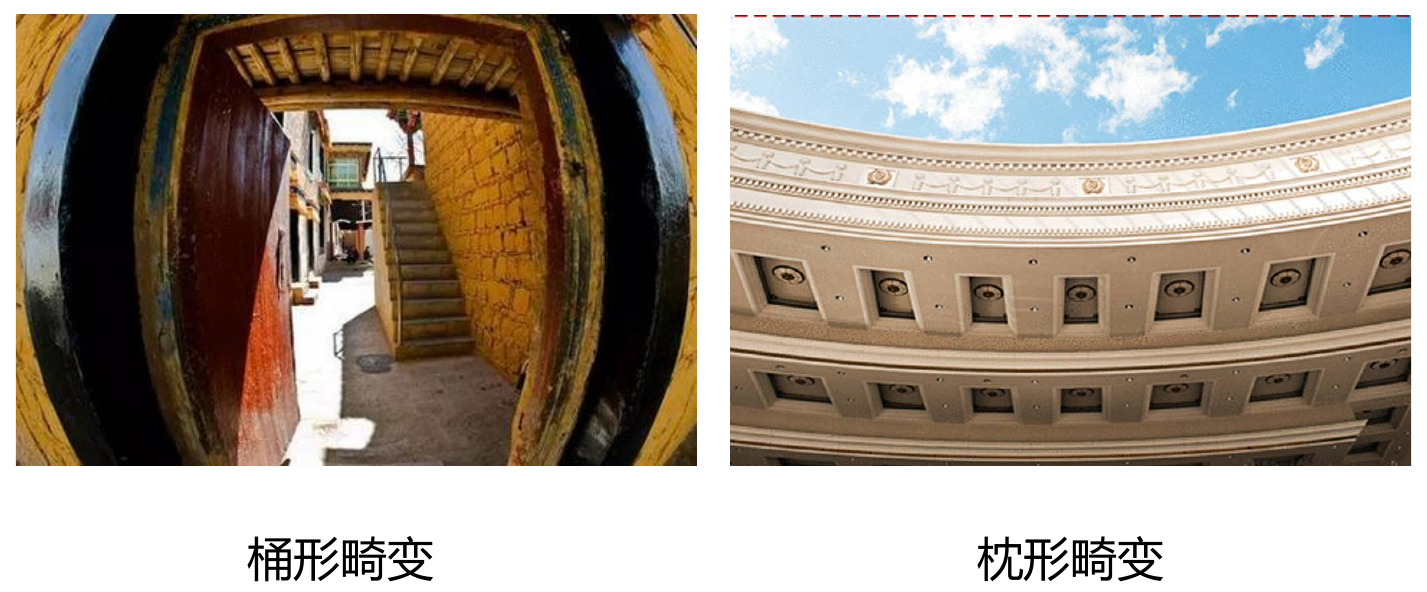
\includegraphics[width=0.88\linewidth]{03-distortion.png}
\caption{桶形畸变与枕形畸变的图像表现。裁自《第3章：图像形成》PDF 第69页。}
\label{fig:rii-distortion}
\end{figure}

\subsection{线性标定、非线性优化与张正友标定法}

\dfn{标定与重投影误差}{相机标定利用一组已知空间坐标及对应像素点，估计内参、外参和畸变参数。将标定点用待估参数投影回像素平面，预测像点与实测像点的像素距离称为重投影误差。其平方和可用作非线性精化的目标函数。}

\begin{enumerate}
\item \textbf{线性标定（DLT）。}令投影矩阵 $M$ 的三行分别为 $\mathbf m_1^\mathsf T,\mathbf m_2^\mathsf T,\mathbf m_3^\mathsf T$，消去齐次比例后，每对匹配点提供两式
\[
(\mathbf m_1-u\mathbf m_3)^\mathsf T\widetilde{\mathbf P}_w=0,\qquad
(\mathbf m_2-v\mathbf m_3)^\mathsf T\widetilde{\mathbf P}_w=0.
\]
$M$ 有 12 个元素，整体比例自由，求一般投影矩阵至少需要 6 对提供足够独立约束的匹配点。点全在同一平面会退化为平面映射问题。
\item \textbf{非线性精化。}可从线性解出发，加入畸变并约束 $R$ 是旋转矩阵，用迭代法最小化 $\sum_i\|(u_i,v_i)-(\widehat u_i,\widehat v_i)\|_2^2$。线性法求初值方便，非线性精化适合描述真实成像。
\item \textbf{张正友标定。}相机设置固定，从多个倾角拍摄已知方格尺寸的平面棋盘，检测角点。取棋盘平面 $Z_w=0$，每幅图满足 $H\sim K[\mathbf r_1\ \mathbf r_2\ \mathbf t]$。利用前两列对应旋转轴的正交性与单位模约束，联合多幅图的单应矩阵求内参，再估各幅外参和畸变，最后精化重投影误差。
\end{enumerate}

\begin{figure}[htbp]
\centering
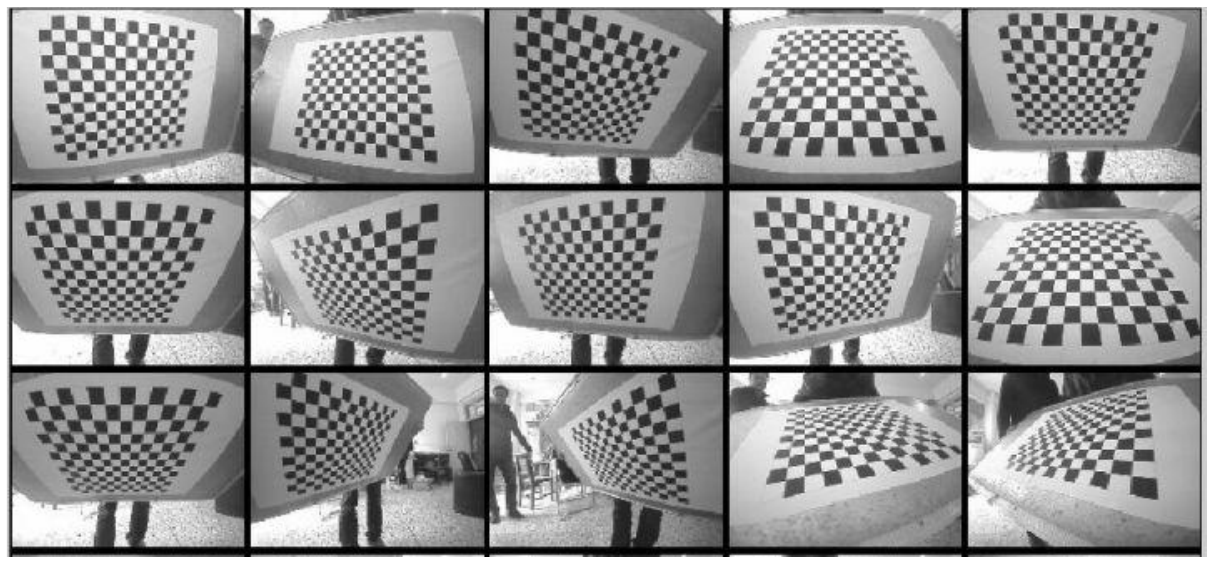
\includegraphics[width=0.75\linewidth]{03-calibration-poses.png}
\caption{相机标定所用的不同倾角与位置的棋盘图像。裁自《第3章：图像形成》PDF 第123页。}
\label{fig:rii-calibration-poses}
\end{figure}

\nt{已知内参时，单个无畸变像素只能确定相机坐标下的一条射线 $\mathbf P_c=Z_cK^{-1}(u,v,1)^\mathsf T$。恢复长度或空间坐标还需要测量平面、深度或多视图等约束。平面标定时应改变棋盘姿态并覆盖视野，留意边缘区域的重投影残差。}

\section{从图像特征到尺寸测量}

平面尺寸测量按\textbf{取感兴趣区域（ROI） $\to$ 去畸变 $\to$ 提取特征 $\to$ 拟合几何模型 $\to$ 转换物理单位}组织。已通过单应矩阵将图像校正到已知平面时，可直接在该平面的物理坐标下算尺寸。若图像已满足均匀比例模型，横纵尺度分别为 $q_x,q_y$ 时，相距 $(\Delta u,\Delta v)$ 的两点距离、由 $N$ 个前景像素组成的区域面积为
\[
\ell=\sqrt{(q_x\Delta u)^2+(q_y\Delta v)^2},\qquad A\approx Nq_xq_y.
\]
倾斜平面或深度变化会改变局部比例。测量齿长等平行边间距时，先将边缘点拟合为共同法向 $(a,b)$ 的两条直线 $ax+by+c_1=0$、$ax+by+c_2=0$，再用 $\lvert c_2-c_1\rvert/\sqrt{a^2+b^2}$ 计算。两条方向向量 $\mathbf v_1,\mathbf v_2$ 的锐夹角可用 $\arccos\bigl(\lvert\mathbf v_1^\mathsf T\mathbf v_2\rvert/(\|\mathbf v_1\|\|\mathbf v_2\|)\bigr)$，若要区分内外角应先确定方向。面积测量可先用连通域标记把各物体分开，再对各域计数。

\textbf{线段端点}可先用 Harris 找角点，再通过拟合边缘精定位。Harris 用窗口平移引起的灰度平方差判断特征，窗口向多个方向移动都产生较大变化时，对应角点。\textbf{Hough 直线检测}用参数式 $\rho=x\cos\theta+y\sin\theta$。单个边缘点在参数空间给出一条曲线；共线的边缘点投票在同一位置聚集。圆的参数为 $(a,b,r)$，每个边缘点对满足 $(x-a)^2+(y-b)^2=r^2$ 的候选投票。已知半径时仅需搜索圆心 $(a,b)$。

\Needspace{5\baselineskip}
\ex{圆轮廓的代数最小二乘拟合}{
在已校正的像素平面中采到四个轮廓点 $(6,2),(0,2),(3,5),(3,-1)$。设圆为
\[
x^2+y^2+A x+B y+C=0.
\]
一般有噪声时，把每点对应的一行 $[x_i\ y_i\ 1]$ 组成矩阵，最小化 $\sum_i[x_i^2+y_i^2+A x_i+B y_i+C]^2$。本例点恰在同一圆上，代入第二点得 $2B+C=-4$；第一点给 $6A+2B+C=-40$，故 $A=-6$；第三点给 $3A+5B+C=-34$，故 $B=-4$、$C=4$；第四点可作校核。配方得到
\[
(x-3)^2+(y-2)^2=9.
\]
圆心为 $(3,2)$，半径为 $3$ 像素。若各方向统一为 $0.20\,\mathrm{mm/pixel}$，物方直径为 $2\times3\times0.20=1.20\,\mathrm{mm}$。代数残差可线性求解，若题目要求最小化实际点到圆弧的距离，应改用几何残差。
}

相机内参和畸变模型为后续视觉控制提供从像素到归一化图像坐标的变换。稳定提取的角点或轮廓可作为图像特征，也可配合目标几何模型估计位姿。

\section{公式速查与自测}

\begin{focusbox}{做题顺序}
\textbf{选型}先确定视野、单像素覆盖、宽高分辨率，再检查靶面与焦距、曝光和照明。\par
\textbf{投影}用 $R\mathbf P_w+\mathbf t$ 计算相机坐标，以 $Z_c$ 归一化，套用畸变模型与 $K$。\par
\textbf{测量}先明确像素与物理平面的对应关系，再找特征、拟合并换算尺寸。
\end{focusbox}

\qs{自测}{
\begin{enumerate}
\item 同时拍摄薄板安装孔和表面划痕，怎样打光？分别说明依据。
\item 已知 $K$、$R$、$\mathbf t$，为什么单个像素无法唯一确定世界点？若目标就在已标定的平面上，怎样求其位置？
\item 靶面为 $8\,\mathrm{mm}\times6\,\mathrm{mm}$，希望在 $\mathrm{WD}=200\,\mathrm{mm}$ 处覆盖约 $100\,\mathrm{mm}\times75\,\mathrm{mm}$，按远距估算应选多大焦距？
\end{enumerate}
}
\noindent\textbf{核对：}（1）背光让孔与板形成轮廓反差。暗场让划痕散射光明显，必要时分时照明拍摄。（2）一个像素给一条反投影射线，将射线与已知平面求交，或求平面单应矩阵的逆变换。（3）从宽或高计算均为 $16\,\mathrm{mm}$。

\chapter{图像处理与特征提取}
\label{chap:rii-image-processing}

\begin{focusbox}{本章复习路线}
从像素出发，先用灰度和邻域运算改善可见性，用几何变换与插值建立像素对应，然后用阈值、边缘或区域法提取目标。对二值掩膜进行形态学处理，再提取尺寸、形状或纹理等特征。\textbf{优先练习}直方图均衡化、双线性插值、滤波与梯度、腐蚀膨胀及开闭运算、OTSU 阈值计算。
\end{focusbox}

本章对应《第4章：图像处理与特征提取》讲义。灰度运算与插值见 PDF 第7--60页，滤波见第61--82页，形态学见第83--97页，分割与缺陷检测见第98--139页。边缘定位、区域面积与测量平面的对应关系见第\ref{chap:rii-image-formation}章。

\section{像素、点运算与直方图}

一幅灰度图可记为 $f(x,y)$，约定 $x$ 为列、$y$ 为行。空间\textbf{采样}决定位置网格的疏密，灰度\textbf{量化}决定幅值的级数。$b$ 位灰度图有 $L=2^b$ 个可用灰度值 $0,\ldots,L-1$。RGB 图像在每个位置记录三分量。亮度描述明暗，反差描述明暗差异，饱和度描述颜色的鲜艳程度。若颜色本身是分类信息，应保留多通道特征。

\dfn{灰度点运算}{对每个输入灰度 $r=f(x,y)$ 使用同一映射，得 $g(x,y)=T[r]$。线性或分段线性拉伸可扩展感兴趣的灰度区间。归一化后令 $0\le r\le1$，伽马变换 $T[r]=r^\gamma$ 在 $0<\gamma<1$ 时提高中间灰度，$\gamma>1$ 时压低中间灰度；对数变换 $T[r]=c\ln(1+r)$ 可展开低灰度区、压缩高灰度区。输出量化时应按题意取整和裁剪。}

\textbf{图像代数与逻辑运算}针对对应像素。例如用乘法或逻辑与保留二值掩膜覆盖的 ROI，用差分观察两幅配准图的变化。多次观测取平均时，若场景保持不变、各帧加性噪声独立且零均值，$M$ 帧平均后噪声方差变为单帧的 $1/M$。计算图像差值前宜转换到有符号或浮点类型。

\subsection{直方图均衡化}

设有 $N$ 个像素，灰度 $k$ 出现 $n_k$ 次。归一化直方图为 $p(k)=n_k/N$，累积分布为 $F(k)=\sum_{i=0}^{k}p(i)$。一种离散均衡化约定为
\[
s_k=\bigl\lfloor (L-1)F(k)\bigr\rfloor .
\]
遍历原图，以 $s_k$ 替代所有灰度为 $k$ 的像素。这个映射保持灰度的非严格次序。离散取整会合并某些灰度级，均衡后的直方图可能仍有峰值。\textbf{直方图规定化}则给出目标分布，按两边的累计概率找最接近的灰度对应关系。

\begin{figure}[htbp]
\centering
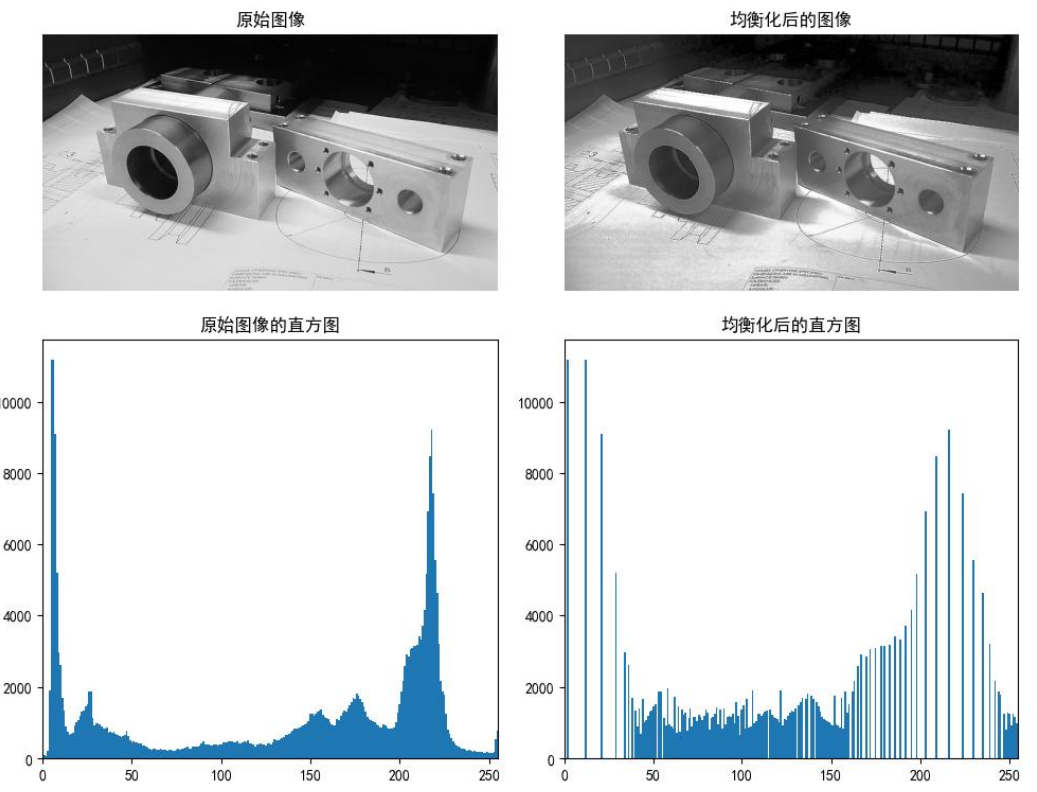
\includegraphics[width=0.75\linewidth]{04-equalization.png}
\caption{均衡化前后的图像和灰度直方图。裁自《第4章：图像处理与特征提取》PDF 第32页。}
\label{fig:rii-hist-equalization}
\end{figure}

\Needspace{5\baselineskip}
\ex{手算四级灰度图的均衡化}{
某 2 位灰度图共 8 像素，灰度 $0,1,2,3$ 的频数分别为 $4,2,1,1$。求按上述向下取整约定得到的映射和输出频数。
\begin{center}
\begin{tabular}{@{}lrrrr@{}}
\toprule
输入灰度 $k$ & $0$ & $1$ & $2$ & $3$ \\
\midrule
$F(k)$ & $4/8$ & $6/8$ & $7/8$ & $8/8$ \\
$(L-1)F(k)$ & $1.5$ & $2.25$ & $2.625$ & $3$ \\
$s_k$ & $1$ & $2$ & $2$ & $3$ \\
\bottomrule
\end{tabular}
\end{center}
输出灰度 $0,1,2,3$ 的频数依次为 $0,4,3,1$，其中输入灰度 1 和 2 都落到输出灰度 2。
}

\nt{有些实现用四舍五入，或先扣除累计分布的最小非零值。手算时先说明取整约定；输出频数要把映射到同一灰度的输入频数相加。直方图只保留各灰度出现次数，仍需位置特征辨别不同形状。}

\section{几何变换和插值}

\subsection{从输出反查输入}

平移、缩放、旋转及剪切可以表示为齐次仿射变换
\[
\begin{bmatrix}x'\\y'\\1\end{bmatrix}
=H\begin{bmatrix}x\\y\\1\end{bmatrix},
\qquad
H=\begin{bmatrix}a&b&t_x\\c&d&t_y\\0&0&1\end{bmatrix}.
\]
若围绕点 $\mathbf c$ 做线性变换 $A$，应使用 $\mathbf p'=A(\mathbf p-\mathbf c)+\mathbf c$。图像的行坐标常向下递增，判断视觉旋转方向时须结合坐标轴方向。
正向变换后取整会使目标网格出现空洞或多点碰撞。对于可逆 $H$，遍历每个输出像素，用 $H^{-1}$ 找其输入坐标，再对原图采样。若反查位置越界，应指定补零、边缘延拓等规则。

\subsection{最近邻、双线性与双三次}

最近邻取离反查位置最近的网格值，适合类别标签。双线性取四个相邻值的加权平均，双三次通常利用 $4\times4$ 邻域，可得到更平滑的结果，代价是计算量更大。图像缩小时，细小结构可能混叠，通常要先适当低通。

\begin{figure}[htbp]
\centering
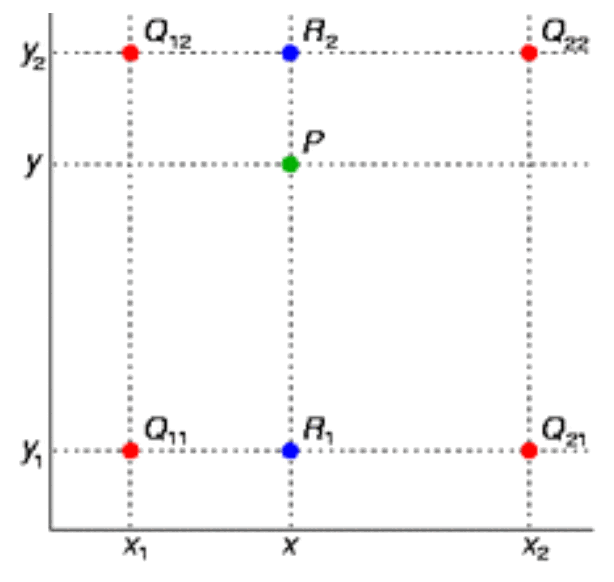
\includegraphics[width=0.45\linewidth]{04-bilinear.png}
\caption{双线性插值的四个网格顶点。先在每一行沿 $x$ 方向插值，再沿 $y$ 方向插值。裁自《第4章：图像处理与特征提取》PDF 第58页。}
\label{fig:rii-bilinear}
\end{figure}

设反查点为 $(i+\alpha,j+\beta)$，$i,j$ 为整数，$0\le\alpha,\beta<1$。先算两行的线性插值
\[
r_0=(1-\alpha)f(i,j)+\alpha f(i+1,j),\qquad
r_1=(1-\alpha)f(i,j+1)+\alpha f(i+1,j+1).
\]
再得 $g=(1-\beta)r_0+\beta r_1$。四个角点权重非负且和为 1，故结果介于这四个值的最小值与最大值之间。

\Needspace{5\baselineskip}
\ex{在反查位置算双线性插值}{
设反查位置为 $(1.25,2.75)$，四个邻点灰度为 $f(1,2)=20$、$f(2,2)=40$、$f(1,3)=60$、$f(2,3)=100$。这里 $\alpha=0.25$、$\beta=0.75$，得
\[
r_0=0.75(20)+0.25(40)=25,\quad r_1=0.75(60)+0.25(100)=70.
\]
所以 $g=0.25(25)+0.75(70)=58.75$。若要求 8 位整数并以四舍五入处理，结果为 59。最近邻选择 $(1,3)$，给出 60。
}

\section{平滑、频域滤波和锐化}

\subsection{空域邻域滤波}

滤波器在滑动窗口内为中心点计算新值。\textbf{均值}等权，\textbf{高斯}让靠近中心的点权重更大，二者都用非负归一化权重，在平坦区域可减弱随机噪声，窗口加大时边缘更易变模糊。高斯核由 $\exp[-(x^2+y^2)/(2\sigma^2)]$ 取样并归一化，$\sigma$ 越大平滑通常越强。\textbf{中值}先排序再取中间值，是非线性滤波；孤立黑白脉冲只要没有占据窗口多数，通常可由它抑制。处理图像边界时应先确定窗口之外的填充规则。

线性邻域运算中，卷积按 $g(x,y)=\sum_{i,j}h(i,j)f(x-i,y-j)$ 相乘求和。若按 $f(x+i,y+j)$ 取邻域，得到相关运算。两者相差一次将核关于中心旋转 $180^\circ$，均值核和中心对称的高斯核旋转后保持原样。手算前应先确认题目约定。

\Needspace{5\baselineskip}
\ex{比较均值、高斯和中值滤波}{
以窗口中心为待更新像素，给定窗口和离散高斯近似核
\[
\begin{bmatrix}20&21&20\\20&255&19\\19&20&20\end{bmatrix},
\qquad
G=\frac1{16}\begin{bmatrix}1&2&1\\2&4&2\\1&2&1\end{bmatrix}.
\]
均值为 $(159+255)/9=46$；用高斯核逐项相乘再相加，得 $(79+160+4\times255)/16=78.6875$；排序为 $19,19,20,20,20,20,20,21,255$，中值为 20。这个窗口的高频异常来自一个孤立亮点，其位置恰在核中心，高斯权重反而让该点对输出影响更大。
}

\subsection{频域滤波与边缘锐化}

令图像横纵尺寸为 $M,N$，二维 DFT 将空间坐标 $(x,y)$ 的信号转换到横纵频率索引 $(u,v)$：
\[
F(u,v)=\sum_{x=0}^{M-1}\sum_{y=0}^{N-1}f(x,y)
\exp\!\left[-2\pi\mathrm{i}\left(\frac{ux}{M}+\frac{vy}{N}\right)\right].
\]
在频域计算 $G=HF$，再作逆 DFT。若频谱经移位使直流位于中心，理想低通取 $H=1$（到中心距离 $D(u,v)\le D_0$）及 $H=0$（$D(u,v)>D_0$）。它能削弱部分高频噪声，同时损失细节。通带边界突变会使空间响应出现振铃。需要用 DFT 实现线性卷积时，还要考虑补零以免引入循环卷积的边界绕回。

\textbf{锐化}可用高频掩模。令 $f_b$ 为平滑图，锐化输出为 $g=f+k(f-f_b)$，其中 $k>0$。也可用四邻接拉普拉斯近似 $\nabla^2f=f_{\text{上}}+f_{\text{下}}+f_{\text{左}}+f_{\text{右}}-4f$，取 $g=f-\lambda\nabla^2f$，$\lambda>0$。若核中心符号反向，回加拉普拉斯响应时的符号也应反向。求梯度或锐化前应留意噪声。

\section{二值图像的形态学}

\subsection{结构元、腐蚀与膨胀}

设 $A$ 是前景为 1 的像素坐标集合，$B$ 为结构元中生效位置相对于锚点的偏移集合。写作 $z+B=\{z+b:b\in B\}$。选好锚点后，用同一坐标约定计算
\[
\begin{aligned}
A\ominus B&=\{z:z+B\subseteq A\},\\
A\oplus B&=\{a+b:a\in A,\ b\in B\}
=\{z:(z+\widehat B)\cap A\ne\varnothing\},\\
\widehat B&=\{-b:b\in B\}.
\end{aligned}
\]
\textbf{腐蚀}可记为“把结构元放到候选锚点，所有有效位置都要落在前景”。\textbf{膨胀}可记为“从每个前景点出发盖出原结构元”，若改为在候选输出点检查是否能碰到输入前景，则使用反射后的结构元 $\widehat B$。对含原点的 $B$，腐蚀缩小或保持前景，膨胀扩大或保持前景。

\subsection{开运算和闭运算}

\[
 A\circ B=(A\ominus B)\oplus B,\qquad
 A\bullet B=(A\oplus B)\ominus B.
\]
开运算先腐蚀后膨胀，可去掉容不下结构元的前景孤点、凸起和细连接；闭运算先膨胀后腐蚀，可填补尺寸和形状与结构元匹配的小裂缝、小空洞，并连接近邻前景。使用同一结构元复做一次开运算或闭运算时，理想集合运算的结果保持不变。

\begin{figure}[htbp]
\centering
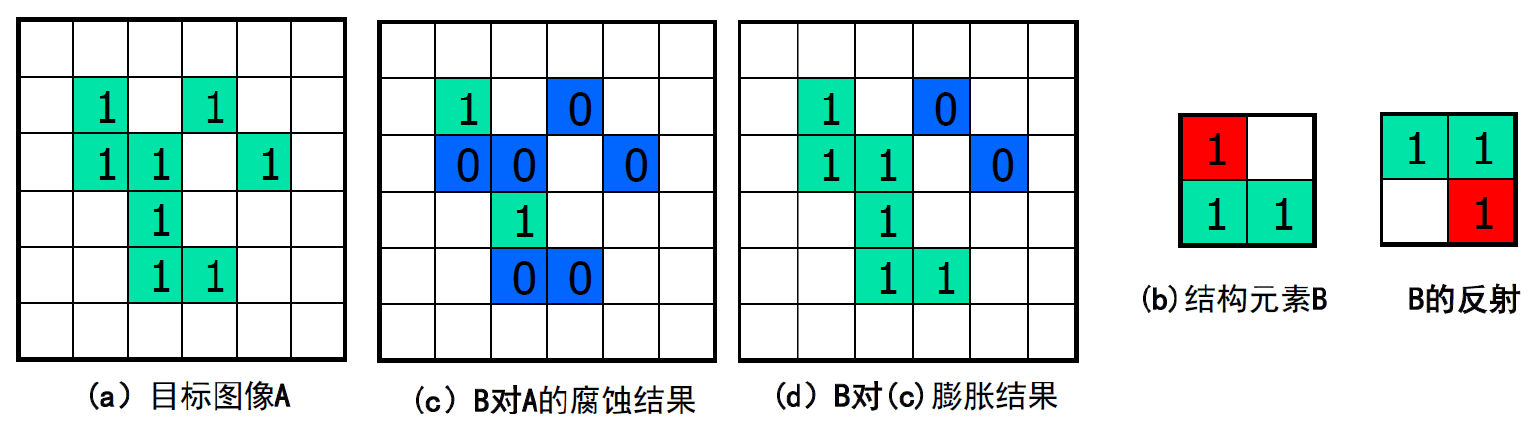
\includegraphics[width=0.96\linewidth]{04-opening.png}
\caption{非对称结构元作用下的开运算。右侧分别为原结构元及其关于锚点的反射。裁自《第4章：图像处理与特征提取》PDF 第95页。}
\label{fig:rii-morph-opening}
\end{figure}

\Needspace{5\baselineskip}
\ex{用集合写出一维开、闭运算}{
取 $A=\{1,2,3,5,6,10\}$，结构元 $B=\{-1,0,1\}$，锚点为 0，窗口在整数线上计算。
\begin{itemize}
\item 只有中心 2 的三个连续位置 $\{1,2,3\}$ 全在 $A$ 中，故 $A\ominus B=\{2\}$。再由中心 2 盖出 $B$，得 $A\circ B=\{1,2,3\}$。
\item 对 $A$ 各点加 $-1,0,1$ 取并集，得 $A\oplus B=\{0,1,\ldots,7\}\cup\{9,10,11\}$。对该集合腐蚀，连续段的两端各退一步，得 $A\bullet B=\{1,2,3,4,5,6,10\}$。
\end{itemize}
开运算去除了短前景段；闭运算补上位置 4，保留了右侧更宽的断开区域。
}

\nt{先看题中前景是黑还是白，再把前景写成集合。结构元的空格不参与覆盖检查。对非对称结构元，若题目要求逐点推膨胀，直接从每个前景位置加 $B$ 通常最方便。}

\section{图像分割：边缘、阈值与区域}

\subsection{梯度边缘与连接}

图像边缘是灰度或纹理在空间上迅速变化的位置。梯度 $\nabla f=(G_x,G_y)^\mathsf T$ 的模 $\sqrt{G_x^2+G_y^2}$ 表示变化强度，角度 $\operatorname{atan2}(G_y,G_x)$ 给出灰度增长最快的方向。在局部直边附近，梯度与边缘切线垂直。实现中也常用 $|G_x|+|G_y|$ 近似强度。对理想阶跃，平滑后在一阶导数幅值的峰附近定位边缘，也可寻找二阶导数的过零点。其他剖面的导数响应见图~\ref{fig:rii-edge-profiles}。

\begin{figure}[htbp]
\centering
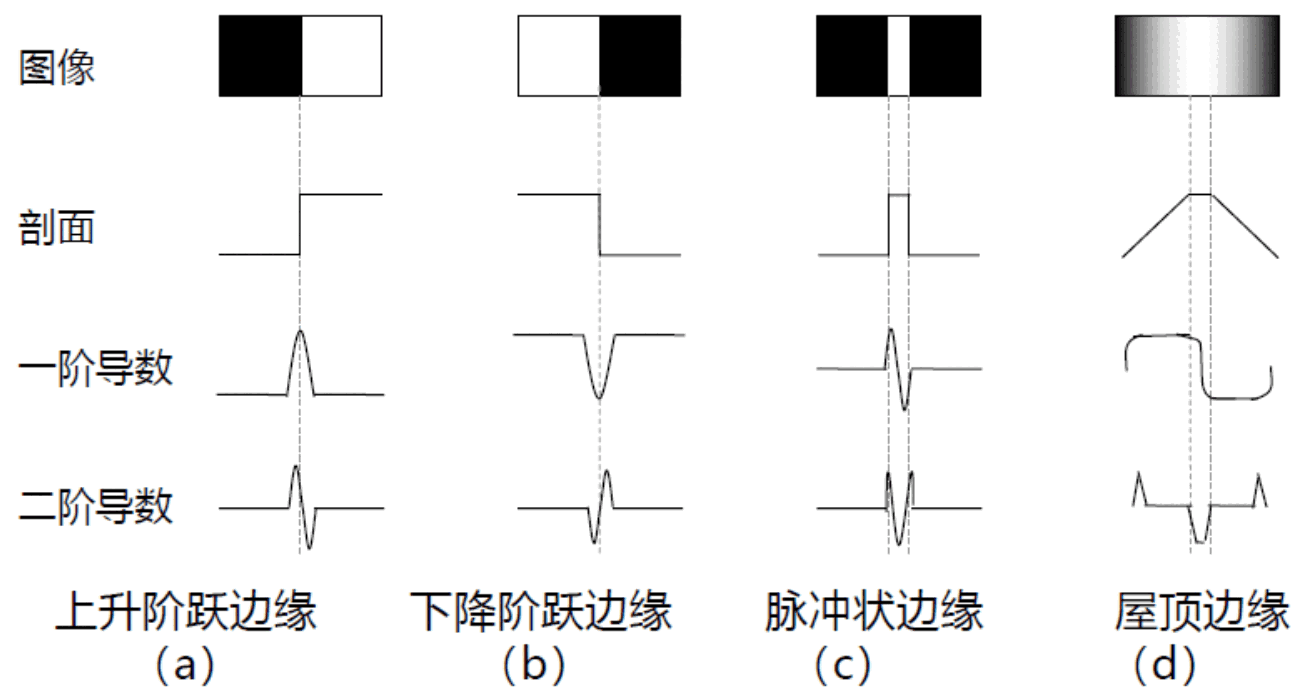
\includegraphics[width=0.86\linewidth]{04-edge-profiles.png}
\caption{四类典型边缘的灰度剖面及导数响应。裁自《第4章：图像处理与特征提取》PDF 第103页。}
\label{fig:rii-edge-profiles}
\end{figure}

以图像的列为 $x$、行为 $y$，若按掩模原顺序与邻域逐项相乘求和（相关），Sobel 算子可取
\[
S_x=\begin{bmatrix}-1&0&1\\-2&0&2\\-1&0&1\end{bmatrix},\qquad
S_y=\begin{bmatrix}-1&-2&-1\\0&0&0\\1&2&1\end{bmatrix}.
\]
Prewitt 用较均匀的横向或纵向平均近似一阶导数，Roberts 在 $2\times2$ 上作对角差分，拉普拉斯给二阶响应。\textbf{Canny}依次做高斯平滑、梯度计算、沿梯度方向非极大值抑制、双阈值与滞后连接，保留与强边缘连通的候选弱边缘。检测得到的边缘可能不连续，若任务为识别几何轮廓，可用 Hough 投票或其他边缘连接方法。

\Needspace{5\baselineskip}
\ex{手算 Sobel 响应并判断边缘方向}{
中心窗口为
$\begin{bmatrix}20&20&80\\20&20&80\\20&20&80\end{bmatrix}$。
按上述掩模，$G_x=(1+2+1)(80-20)=240$，$G_y=0$，梯度模为 240。灰度沿列坐标正向增长，边缘切线沿行坐标方向，对应图像中的竖直边缘。
}

\subsection{全局阈值与 OTSU}

单阈值分割将图像划分为 $f\le t$ 和 $f>t$ 两类，哪一类为前景由任务决定。目标和背景灰度分布分离时，全局阈值计算简单。照明随位置明显变化时，可依据局部窗口统计量设置自适应阈值 $t(x,y)$。

设候选阈值为 $t$，分别计算两类权重 $\omega_0,\omega_1$ 和类均值 $\mu_0,\mu_1$：
\begin{align*}
\omega_0&=\sum_{k=0}^t p(k),& \omega_1&=1-\omega_0,\\
\mu_0&=\frac{\sum_{k=0}^t k p(k)}{\omega_0},&
\mu_1&=\frac{\sum_{k=t+1}^{L-1} k p(k)}{\omega_1}.
\end{align*}
以 $\mu_T=\omega_0\mu_0+\omega_1\mu_1$ 表示整图均值，类间方差为
\[
\sigma_B^2(t)=\omega_0(\mu_0-\mu_T)^2+\omega_1(\mu_1-\mu_T)^2
=\omega_0\omega_1(\mu_0-\mu_1)^2.
\]
\textbf{OTSU（大津法）}枚举使两类皆非空的 $t$，取类间方差最大的阈值。将总平方偏差按类展开，可得总方差等于类内方差与类间方差之和，所以最大化类间方差同时最小化加权类内方差。最佳阈值若并列，应按题意作出取值约定，空灰度段中多个阈值可能对应同一划分。

\Needspace{5\baselineskip}
\ex{给定直方图求 OTSU 阈值}{
设只可能出现灰度 $0,1,2,3$，且每级各有两个像素。枚举 $t=0,1,2$：
\begin{center}
\begin{tabular}{@{}crrrrc@{}}
\toprule
$t$ & $\omega_0$ & $\omega_1$ & $\mu_0$ & $\mu_1$ & $\sigma_B^2$ \\
\midrule
0 & $1/4$ & $3/4$ & $0$ & $2$ & $3/4$ \\
1 & $1/2$ & $1/2$ & $1/2$ & $5/2$ & $1$ \\
2 & $3/4$ & $1/4$ & $1$ & $3$ & $3/4$ \\
\bottomrule
\end{tabular}
\end{center}
例如 $t=1$ 时，低灰度类由 0 和 1 组成，均值 $\mu_0=(0/4+1/4)/(1/2)=1/2$；高类均值同理为 $5/2$。最大类间方差取在 $t=1$，分割为 $\{0,1\}$ 和 $\{2,3\}$。
}

\subsection{区域生长、分裂与合并}

\textbf{区域生长}由种子开始，在四邻域或八邻域中把满足一致性判据的邻点并入区域，直至没有新点可加入。判据可用与种子强度之差，也可用与当前区域均值之差。阈值过小会漏收像素，过大可能穿过边界扩张；种子选择、邻接规则和冲突处理都影响结果。在只沿行列接触的四邻域下，两个角接触的像素各自独立；八邻域中对角接触也算连通。

\textbf{区域分裂与合并}选择区域一致性谓词，例如灰度标准差不超过阈值。用四叉树将不满足条件的块继续分裂，再依据合并判据将相邻且足够相似的区域合并。阈值分割主要看像素强度，边缘分割看突变位置，区域法还使用空间连通性。

\section{缺陷检测与特征分类}

\subsection{从差分图到特征向量}

设待测图为 $I$，无缺陷模板为 $I_0$。固定光照或完成亮度校正，并将两幅图配准后，可令 $D(x,y)=|I(x,y)-I_0(x,y)|$，阈值化得到疑似缺陷。之后用开闭运算清理掩膜，按连通域提取面积、长宽、位置和灰度统计，再按公差筛选。模板错位会在正常轮廓附近生成高差值，因此差分前的配准会直接影响可靠性。

\textbf{特征提取}将图像或感兴趣区域转换为灰度、梯度、几何、直方图或纹理量。\textbf{特征选择}从已有特征中保留有辨别力的分量；若用主成分分析把多维特征投影到低维，新分量由原特征组合而来。在比较单独提取的直方图时，先确认像素数是否需要归一化，再看分布差异；若缺陷判定依赖位置，应结合 ROI、边缘或局部特征。

\subsection{K 近邻与朴素贝叶斯}

\textbf{K 近邻（KNN）}把待判样本与训练样本的特征向量比较，按距离排序，取最近的 $K$ 个样本投票。距离可用欧氏距离 $\bigl[\sum_i(x_i-z_i)^2\bigr]^{1/2}$ 或曼哈顿距离 $\sum_i|x_i-z_i|$。若把面积、长度、灰度等数值尺度不同的量放在同一向量中，应先处理量纲与尺度。$K$ 太小对噪声样本敏感，太大则可能将具有不同性质的样本混入邻居。

\textbf{朴素贝叶斯}由先验概率和类条件似然比较后验。给定特征 $\mathbf x=(x_1,\ldots,x_d)$，在各特征在给定类别 $C$ 时条件独立的假设下，
\[
P(C\mid\mathbf x)\propto P(C)\prod_{j=1}^{d}P(x_j\mid C).
\]
分母 $P(\mathbf x)$ 对各类别相同，分类时比较右侧得分即可。若数据表给的是先验和似然，不能直接把似然当作后验。

\Needspace{9\baselineskip}
\ex{用两项特征判别缺陷}{
设工件缺陷先验为 $0.10$，正常先验为 $0.90$。观察到“面积偏大”和“灰度差偏大”，这两事件在给定类别时条件独立。两事件在缺陷类中的条件概率为 $0.80,0.70$，在正常类中为 $0.10,0.20$。计算类别得分：
\[
s_{\text{缺陷}}=0.10\times0.80\times0.70=0.056,\qquad
s_{\text{正常}}=0.90\times0.10\times0.20=0.018.
\]
故按最大后验概率判缺陷。归一化后缺陷概率为 $0.056/(0.056+0.018)\approx0.757$。
}

\Needspace{8\baselineskip}
\section{公式速查与自测}

\begin{focusbox}{常见题型的第一步}
\textbf{灰度与插值}先确定灰度级数和取整约定，几何题先确定变换方向与像素坐标。\par
\textbf{空间滤波}先写中心窗口，排序取中值或按权重逐项相乘。\par
\textbf{形态学与分割}先明确前景、结构元锚点和邻域，OTSU 要排除空类候选，梯度题分清梯度方向和边缘方向。\par
\textbf{缺陷检测}先保证模板和待测图在位置与亮度上可比，再计算差异和区域特征。
\end{focusbox}

\qs{自测}{
\begin{enumerate}
\item 二值标签图做放大时应优先考虑哪种插值？若是灰度图且希望过渡连续，又可选择什么？
\item 得到一张黑底白字的二值图，白字旁有孤立白点，笔画里有小黑孔。分别可用哪种形态学运算？
\item 对一幅梯度满足 $G_x=0$、$G_y>0$ 的局部图像，边缘走向如何？若图中有高斯噪声，应如何提高梯度的稳定性？
\item 两张图像的灰度直方图完全相同，能否只据此判定工件轮廓一致？用模板做差前应检查什么？
\end{enumerate}
}
\noindent\textbf{核对：}（1）标签用最近邻，灰度图可用双线性。（2）对前景白色用开运算去白点，用闭运算填黑孔，并按尺寸选结构元。（3）梯度沿行坐标正向，边缘沿列坐标方向，求梯度前可作高斯平滑。（4）直方图缺少像素位置信息。应检查配准和照明的一致性。

\chapter{机器人的控制}
\label{ch:robot-control}

\begin{focusbox}{复习重点}
会从电枢电压与机械力矩平衡写出单关节传递函数，按特征方程选取位置和速度增益；会从动力学方程推出计算力矩、关节和笛卡尔阻抗，以及力/位混合控制。做接触控制题时，先选约束坐标系、画出力方向，再写控制律。PID 仿真、上述控制器设计和两种视觉伺服的比较见\hyperref[hw:robot-control]{控制部分课后作业精解}。
\end{focusbox}

\section{单关节电机建模与位置反馈}

\subsection{传动折算与开环模型}
取讲义的传动比约定 $n=z_m/z_L=\theta_L/\theta_m$，减速时 $0<n<1$。若设备铭牌把减速比写为 $i=\theta_m/\theta_L$，则 $n=1/i$；第\ref{chap:actuators}章用 $N=1/n$。由动能 $\tfrac12J_L\dot\theta_L^2=\tfrac12n^2J_L\dot\theta_m^2$ 和黏性耗散的同类关系，电机轴上的等效量为
\[
J_{\mathrm{eff}}=J_m+n^2J_L,\qquad f_{\mathrm{eff}}=f_m+n^2f_L.
\]
理想传动下 $\tau_m\dot\theta_m=\tau_L\dot\theta_L$，所以负载力矩折算到电机侧乘 $n$，负载惯量折算乘 $n^2$。例：$J_m=0.01\,\mathrm{kg\,m^2}$、$J_L=2\sim8\,\mathrm{kg\,m^2}$、$n=1/40$，则 $J_{\mathrm{eff}}=0.01125\sim0.015\,\mathrm{kg\,m^2}$（讲义第12页）。

令 $u_a,i_a,R_a,L_a$ 分别为电枢电压、电流、电阻、电感，$k_a$ 为力矩系数，$k_b$ 为反电势系数。把阻碍正转的扰动在电机侧记为 $d_m$，方程为
\[
\begin{aligned}
 u_a &= R_a i_a+L_a\dot i_a+k_b\dot\theta_m,\\
 J_{\mathrm{eff}}\ddot\theta_m+f_{\mathrm{eff}}\dot\theta_m &=k_ai_a-d_m,\qquad \theta_L=n\theta_m.
\end{aligned}
\]
令 $d_m=0$，在零初值下消去 $I_a$，得到负载角位移的开环模型
\[
G(s)=\frac{\Theta_L(s)}{U_a(s)}
 =\frac{n k_a}{s[(R_a+L_a s)(J_{\mathrm{eff}}s+f_{\mathrm{eff}})+k_a k_b]}.
\]
当电气动态远快于机械动态时，可令 $L_a\approx0$。定义 $\gamma=R_a f_{\mathrm{eff}}+k_a k_b$，简化为 $G(s)=n k_a/[s(R_a J_{\mathrm{eff}}s+\gamma)]$。若输出取角速度，则分子多乘一个 $s$。反电势使 $\gamma$ 中多出 $k_a k_b$，它与机械黏性项共同提供速度阻尼。

\subsection{闭环传递函数、阻尼与稳态误差}
以 $r=\theta_L^d$、$e=r-\theta_L$，按讲义用 $u_a=(k_p e+k_v\dot e)/n$。接回 $\Theta_L=GU_a$，得到
\[
\frac{\Theta_L(s)}{R(s)}=\frac{k_a(k_p+k_vs)}{D(s)},\qquad
D(s)=R_aJ_{\mathrm{eff}}s^2+(\gamma+k_ak_v)s+k_ak_p.
\]
\begin{figure}[H]
    \centering
    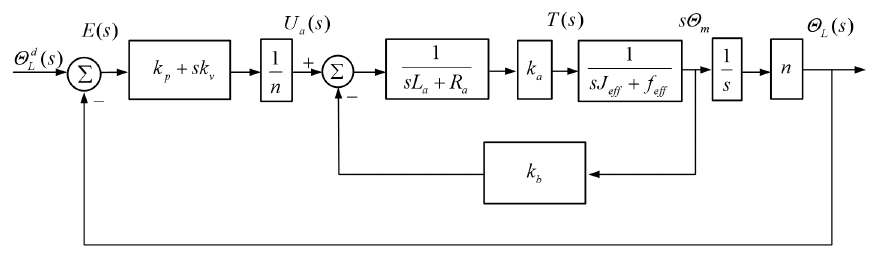
\includegraphics[width=0.95\linewidth]{05-joint-feedback.png}
    \caption{单关节位置、速度误差反馈及电机反电势内反馈。截取自第5章讲义 PDF 第17页。}
\end{figure}
比较 $D(s)/(R_aJ_{\mathrm{eff}})=s^2+2\zeta\omega_n s+\omega_n^2$ 各项系数得
\[
  \omega_n=\sqrt{\frac{k_a k_p}{R_aJ_{\mathrm{eff}}}},\qquad
  \zeta=\frac{\gamma+k_a k_v}{2\sqrt{R_aJ_{\mathrm{eff}}k_a k_p}}.
\]
给定 $\omega_n,\zeta$，先求 $k_p=R_aJ_{\mathrm{eff}}\omega_n^2/k_a$，再求 $k_v=(2\zeta\omega_n R_aJ_{\mathrm{eff}}-\gamma)/k_a$。$\zeta=1$ 时特征根重合，$0<\zeta<1$ 为欠阻尼，$\zeta>1$ 为过阻尼。读阶跃曲线还需看传递函数的零点，例如误差微分会在分子引入 $k_vs$，阶跃参考同时带来理想微分冲击。用 $u_a=[k_p(r-\theta_L)-k_v\dot\theta_L]/n$，分母相同、分子只有 $k_a k_p$。讲义用 $\omega_n\leq\omega_r/2$ 作避开结构共振的设计约束，$\omega_r$ 为结构共振频率。

用 $L_a=0$ 的模型保留 $d_m$，有 $D(s)\Theta_L=k_a(k_p+k_vs)R-nR_aD_m$，所以
\[
 E(s)=\frac{(R_aJ_{\mathrm{eff}}s^2+\gamma s)R(s)+nR_aD_m(s)}{D(s)}.
\]
闭环稳定时，对阶跃参考 $R=A/s$ 及恒定阻力矩 $D_m=d_0/s$，终值定理给出 $e_{\mathrm{ss}}=nR_a d_0/(k_a k_p)$。若 $d_0=0$，单位负反馈的角位置开环有一个积分环节，阶跃参考无静差。斜率为 $A$ 的斜坡参考 $R=A/s^2$ 则另有跟踪滞后 $A\gamma/(k_a k_p)$（采用误差微分）。重力等已知力矩可在电机侧前馈补偿，剩余扰动决定相应的静差。

\ex{按二阶极点选伺服增益}{若 $R_a=2$、$J_{\mathrm{eff}}=0.02$、$\gamma=0.11$、$k_a=0.1$，取 $\omega_n=4\,\mathrm{rad/s}$、$\zeta=1$，则 $k_p=0.04\times16/0.1=6.4$，$k_v=(0.04\times8-0.11)/0.1=2.1$。特征多项式变为 $s^2+8s+16=(s+4)^2$。只取 $k_p$ 时阻尼比为 $0.11/0.32\approx0.344$，增加速度反馈在模型中补足了阻尼。}

\section{控制规律分解与计算力矩}
\label{sec:computed-torque}
单轴模型 $m\ddot x+b\dot x+kx=f$ 有两种解法。直接按位移、速度反馈 $f=-k_px-k_v\dot x$，闭环的实际阻尼和刚度为 $b+k_v$、$k+k_p$。采用 $f=\alpha u+\beta$ 时，选 $\alpha=m,\ \beta=b\dot x+kx$ 得 $\ddot x=u$。令 $e=x_d-x$，用 $u=\ddot x_d+k_v\dot e+k_pe$ 即得 $\ddot e+k_v\dot e+k_p e=0$。在后一种写法中，$k_p=\omega_n^2$ 是归一化系数，定点附近抵抗外力的实际刚度为 $m k_p$。

多关节机械臂写作 $M(q)\ddot q+h(q,\dot q)=\tau$，其中 $M$ 是对称正定的惯性矩阵，$h$ 汇总科氏力、离心力、重力与摩擦等模型项。令 $e=q_d-q$，计算力矩法用
\[
\begin{aligned}
 u&=\ddot q_d+K_v\dot e+K_pe,\\
 \tau&=\widehat M(q)u+\widehat h(q,\dot q).
\end{aligned}
\]
帽号表示计算使用的模型。模型精确且无外扰时 $\ddot q=u$，所以 $\ddot e+K_v\dot e+K_pe=0$；取正对角增益，各轴化为独立的二阶误差系统，可令 $k_{p,i}=\omega_{n,i}^2$、$k_{v,i}=2\zeta_i\omega_{n,i}$。参考加速度提供前馈，误差反馈校正初始偏差与模型残差。模型参数不准时，剩余项随构型和速度变化，各轴可能再次耦合。

\section{约束坐标系与直接力控制}
\label{sec:force-control}
\dfn{自然约束与人工约束}{几何接触限制运动，环境也限制可传递的力，这些由环境决定，称为自然约束。人工约束指定机器人还可选择的量，例如沿光滑台面切向走给定轨迹、沿台面法向维持给定压力。约束坐标系以环境几何或任务方向选轴，可固定在环境中，也可随任务更新。}

\begin{figure}[H]
    \centering
    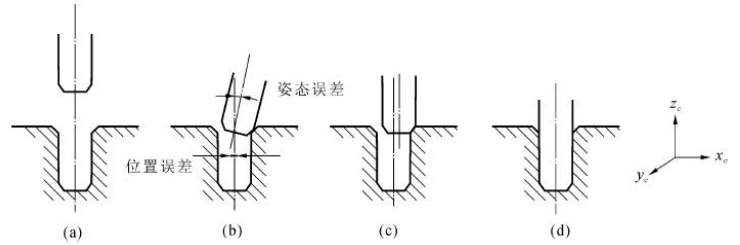
\includegraphics[width=0.76\linewidth]{05-peg-in-hole.png}
    \caption{圆棒入孔的接近、接触、对准、插入四个阶段。接触状态改变时，应重判自由方向与受约束方向。截取自第5章讲义 PDF 第47页。}
\end{figure}

单轴直接力控制以弹性接触为例。取压入为正，$f_e=k_e x$ 是机器人施于环境的力，$f$ 为驱动作用，$f_{\mathrm{dis}}$ 为额外阻力。由 $m\ddot x=f-f_e-f_{\mathrm{dis}}$ 得
\[
  f=\frac{m}{k_e}\ddot f_e+f_e+f_{\mathrm{dis}}\quad(k_e>0).
\]
以 $e_f=f_d-f_e$，取 $u_f=\ddot f_d+k_{vf}\dot e_f+k_{pf}e_f$，可以用 $f=(m/k_e)u_f+f_e$ 补偿接触弹力，或用 $f=(m/k_e)u_f+f_d$ 作参考力前馈。第一种误差方程为 $\ddot e_f+k_{vf}\dot e_f+k_{pf}e_f=(k_e/m)f_{\mathrm{dis}}$；第二种把刚度项系数改为 $k_{pf}+k_e/m$。常值扰动下，在闭环稳定时，后者稳态误差为 $f_{\mathrm{dis}}/(1+mk_{pf}/k_e)$。这两种式子只适用于接触模型成立的阶段，推导与增益选择见\hyperref[hw:control-10-3]{教材题 10.3}。

\section{顺应、阻抗与导纳}
\label{sec:robot-impedance}
\dfn{顺应与阻抗}{顺应描述外力引起的位移变化。被动顺应靠机械柔性，例如远中心柔顺装置 RCC 帮助插装对准；主动顺应通过控制设定刚度。阻抗在弹簧项之外还规定惯性和阻尼，描述交互的动态过程。}
局部小位移下 $\delta x=J\delta q$，由虚功 $f^{\mathsf T}\delta x=\tau^{\mathsf T}\delta q$ 得 $\tau=J^{\mathsf T}f$。因此定点无预载（或冻结 $J$）时，末端刚度 $K_x$ 对应的关节空间增量刚度为 $K_q=J^{\mathsf T}K_xJ$。接触通常取较低法向刚度缓冲碰撞，保留合适的切向刚度以跟踪轨迹。

\begin{figure}[H]
    \centering
    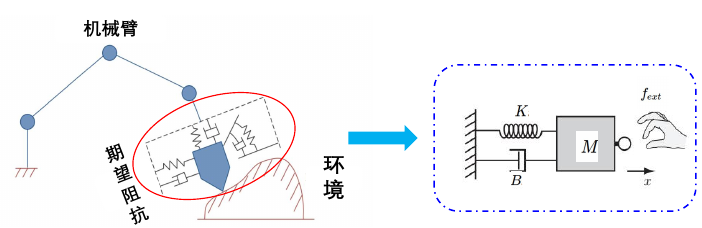
\includegraphics[width=0.79\linewidth]{05-impedance-model.png}
    \caption{用虚拟质量、阻尼和弹簧描述末端与环境的交互。截取自第5章讲义 PDF 第69页。}
\end{figure}
令 $\Delta x=x-x_d$，$f_{\mathrm{ext}}$ 为环境施于机器人的外力，典型目标模型为
\[
  M_d\Delta\ddot x+B_d\Delta\dot x+K_d\Delta x=f_{\mathrm{ext}}.
\]
$M_d,B_d,K_d$ 分别为期望惯量、阻尼、刚度，通常选为正定矩阵。若题目用 $e_x=x_d-x$，上式右端随之改为 $-f_{\mathrm{ext}}$。令 $Z_x(s)=F_{\mathrm{ext}}(s)/\Delta X(s)=M_d s^2+B_d s+K_d$（零初值），即讲义按位移定义的阻抗，也称动态刚度；按速度定义的机械阻抗为 $Z_x(s)/s$。单轴恒力平衡位移为 $f_{\mathrm{ext}}/K_d$，$M_d$ 和 $B_d$ 在此平衡式中消失。单轴瞬态的 $\omega_n=\sqrt{K_d/M_d}$、$\zeta=B_d/(2\sqrt{M_dK_d})$ 可用来设计过渡过程。

\begin{center}
\small
\begin{tabularx}{\linewidth}{@{}p{0.16\linewidth}XX@{}}
\toprule
控制方式 & 从测量到指令 & 总体实现 \\
\midrule
阻抗控制 & 位姿偏差、速度等 $\to$ 调节作用力/力矩 & 常与力矩或电流内环配合 \\
导纳控制 & 外力或力误差 $\to$ 通过二阶模型生成运动修正 & 常与位置或速度内环配合 \\
\bottomrule
\end{tabularx}
\end{center}
若对虚拟阻抗模型求逆，就有 $\Delta X=Z_x^{-1}F_{\mathrm{ext}}$。导纳实现将该二阶方程积分，得到运动参考供内环跟踪。关节空间把 $x,f_{\mathrm{ext}}$ 换为 $q,\tau_{\mathrm{ext}}$；笛卡尔空间还需用 $\dot x=J\dot q$、$\ddot x=J\ddot q+\dot J\dot q$ 或任务空间逆动力学。具体推导见\hyperref[hw:control-3]{作业第3题}。

\section{直接力/位置混合控制}
\label{sec:robot-hybrid}
在约束坐标系中选 $S_p$ 投影到位置控制方向。使用正交轴时，$S_p$ 为对角选择矩阵，位置轴取 $1$，余项取 $0$。力方向用 $S_f=I-S_p$，有 $S_pS_f=0$。在同一坐标系、同一广义量中合成命令，例如均写为笛卡尔广义力时
\[
 F_{\mathrm{cmd}}=S_p F_{\mathrm{pos}}+S_f F_{\mathrm{force}},\qquad
 \tau_{\mathrm{cmd}}=J_c^{\mathsf T} F_{\mathrm{cmd}}+\tau_{\mathrm{model}}.
\]
$J_c$ 将关节速度映射到该约束坐标系中的末端速度。上式给出信号分配，动力学耦合须由模型补偿或在控制器中考虑。纯位置控制的极端情形是 $S_p=I$；光滑台面接触中，约束系的两个切向分量由位置支路控制，法向分量由力支路控制。讲义例以 $y$ 为法向，则 $S_p=\operatorname{diag}(1,0,1)$，$S_f=\operatorname{diag}(0,1,0)$。位置矢量与力矢量须统一表达在约束系并分别形成误差，混合时再把换算后的同类指令相加。

\nt{自然约束与控制目标成对出现。光滑面切向不能承担理想摩擦力，可沿切向跟踪位置；法向运动受阻，可控制压力。接近接触点时先执行自由空间轨迹，确认建立接触后再启用法向力支路。}

\section{视觉伺服：从视觉特征误差生成运动}
\label{sec:visual-servo}
视觉伺服反复采集图像、估计误差并下发相机或机械臂速度。PBVS（基于位置）用从图像重建的三维相对位姿构造误差。IBVS（基于图像）用像点、线或其他图像特征构造误差。两者都是图像进入反馈环，差别在反馈误差所在的空间。

用相机速度旋量 $v_c=(v_x,v_y,v_z,\omega_x,\omega_y,\omega_z)^{\mathsf T}$，特征运动为 $\dot s=L_s v_c$，$L_s$ 称为交互矩阵。常用速度律 $v_c=-\lambda\widehat L_s^+(s-s_d)$，其中 $+$ 表示伪逆。若交互矩阵精确且在目标附近具有足够的秩，特征误差沿可控方向衰减。手眼结构还需将相机速度变换到机器人控制坐标系，再用机器人雅可比求关节速度。点特征的交互矩阵和 PBVS/IBVS 的优缺点见\hyperref[hw:control-5]{作业第5题}。

\section{考前自测}
\qs{控制模型与符号}{\begin{enumerate}
  \item 如果把传动比改记为 $i=40$，如何将负载惯量、负载力矩折算到电机轴？
  \item 位置误差微分与角速度负反馈的闭环特征多项式相同。为什么两者的阶跃响应仍可能不同？
  \item 目标误差定义从 $x-x_d$ 改成 $x_d-x$，外力方向保持原约定，阻抗等式应如何改写？
  \item 机器人沿无摩擦斜面滑动并保持法向压力，应如何写选择矩阵？
\end{enumerate}}
\noindent\textbf{核对}　(1) 分别除以 $i^2$、$i$。(2) 参考的微分通道改变分子，引入零点；理想阶跃会产生微分冲击。(3) 右端变为 $-f_{\mathrm{ext}}$。(4) 在法向为第三轴的约束系中，$S_p=\operatorname{diag}(1,1,0)$，$S_f=\operatorname{diag}(0,0,1)$。

\chapter*{控制部分课后作业精解}
\phantomsection
\addcontentsline{toc}{chapter}{控制部分课后作业精解}
\label{hw:robot-control}
\markboth{控制部分课后作业精解}{控制部分课后作业精解}

依据《控制部分 课后作业》，按编号讲解第1至5题，再解析嵌在文档中的五道教材题（《机器人学：建模、控制与视觉》印刷页262--263、280）。第1至4题的仿真采用本册选定的模型参数，源码为 \texttt{scripts/control\_homework.m}，用 MATLAB 自带的 \texttt{ode45} 和绘图函数即可复现。图中的反馈量、符号和数值按各题说明取用。

\noindent\textbf{题目索引}　\hyperref[hw:control-1]{1. PID}　\hyperref[hw:control-2]{2. 单关节位置反馈}　\hyperref[hw:control-3]{3. 阻抗}　\hyperref[hw:control-4]{4. 力/位混合}　\hyperref[hw:control-5]{5. 视觉伺服}\\
\phantom{\textbf{题目索引}　}\hyperref[hw:control-9-1]{9.1}　\hyperref[hw:control-9-4]{9.4}　\hyperref[hw:control-9-10]{9.10}　\hyperref[hw:control-9-15]{9.15}　\hyperref[hw:control-10-3]{10.3}

\section*{第1题　用二阶对象比较 PID 参数}
\label{hw:control-1}
\qs{题意}{选一个二阶开环系统，在 MATLAB/Simulink 中仿真 PID 控制，讨论三个增益 $K_P,K_I,K_D$ 对响应的影响。}
\textbf{建模与控制律}　取 $G(s)=1/(s^2+2s+4)$，即 $\ddot x+2\dot x+4x=u$。以 $e=r-x$，理想并联 PID 写成 $u=K_Pe+K_I\int e\,\mathrm dt+K_D\dot e$。在单位负反馈、零初值下，闭环为
\[
  \frac{X}{R}=\frac{K_Ds^2+K_Ps+K_I}{s^3+(2+K_D)s^2+(4+K_P)s+K_I}.
\]
为避免阶跃参考引起理想微分冲击，仿真采用测量量微分 $u=K_P(1-x)+K_I z-K_D\dot x$，$\dot z=1-x$。此时传递函数分母与上式相同，分子改为 $K_Ps+K_I$。当 $K_I>0$ 时，由三阶 Routh 判据，稳定条件为
\[
  2+K_D>0,\quad 4+K_P>0,\quad K_I>0,\quad (2+K_D)(4+K_P)>K_I.
\]
$K_I=0$ 时闭环化简为二阶，按二阶分母判稳。无积分的稳定闭环对单位阶跃有 $x_{\mathrm{ss}}=K_P/(4+K_P)$，有积分且稳定时 $x_{\mathrm{ss}}=1$。

\textbf{仿真读数与解释}　零初值，参考为 $1\,\mathrm m$，按 $0.01\,\mathrm s$ 采样输出。峰值是 $0$ 至 $12\,\mathrm s$ 的最大采样值。
\begin{center}
\small
\begin{tabular}{@{}lrrrrr@{}}
\toprule
控制 & $K_P$ & $K_I$ & $K_D$ & 峰值/$\mathrm m$ & $x(12\,\mathrm s)/\mathrm m$ \\
\midrule
P   & 4  & 0 & 0 & 0.6525 & 0.5000 \\
P   & 12 & 0 & 0 & 1.0833 & 0.7500 \\
PI  & 12 & 8 & 0 & 1.2858 & 0.9996 \\
PD  & 12 & 0 & 6 & 0.7500 & 0.7500 \\
PID & 12 & 8 & 6 & 1.0277 & 1.0000 \\
\bottomrule
\end{tabular}
\end{center}
\begin{itemize}[nosep]
  \item $K_P$ 增大，当下误差产生更大的驱动，二阶模型的自然频率 $\sqrt{4+K_P}$ 增大，静差减小。在本例阻尼系数固定的前两行，阻尼比随之降低，峰值增大。
  \item $K_I$ 累积误差，闭环稳定且无持续饱和时消除常值参考的静差。积分引入额外动态，本例 PI 的峰值增大。积分增益过大可使 Routh 条件失效。
  \item $K_D$ 对快速运动提供制动。本例 PD 的分母是 $s^2+8s+16=(s+4)^2$，临界阻尼且无超调。PD 仍有静差；PID 与 PI 比较时，$K_D$ 降低了峰值。实际微分需考虑测量噪声和滤波。
\end{itemize}

\section*{第2题　机械臂单关节位置反馈}
\label{hw:control-2}
\qs{题意}{推导机械臂单关节位置反馈，画控制框图、求闭环传递函数，并在 MATLAB/Simulink 中仿真验证。}
按第\ref{ch:robot-control}章的电枢与电机轴模型，取 $L_a\approx0$、$\gamma=R_a f_{\mathrm{eff}}+k_a k_b$、$n=\theta_L/\theta_m$。用角速度负反馈 $u_a=[k_p(r-\theta_L)-k_v\dot\theta_L]/n$，其信号流如下。电机反电势内反馈已包含在 $G(s)$ 的 $\gamma$ 中。

\begin{center}
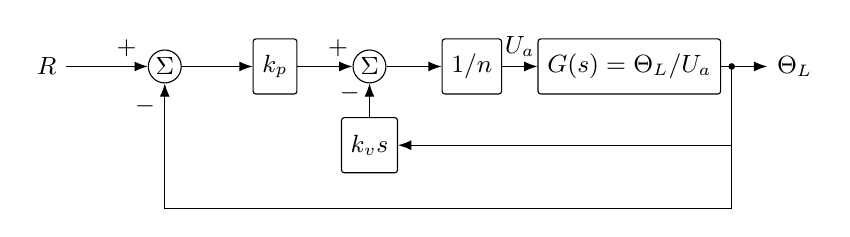
\begin{tikzpicture}[>=Latex, font=\small, block/.style={draw, rounded corners=1pt, align=center, minimum height=7mm}, sum/.style={draw, circle, inner sep=1pt}]
  \node (r) at (0,0) {$R$};
  \node[sum] (e) at (1.5,0) {$\Sigma$};
  \node[block] (p) at (2.9,0) {$k_p$};
  \node[sum] (u) at (4.1,0) {$\Sigma$};
  \node[block] (gear) at (5.4,0) {$1/n$};
  \node[block] (plant) at (7.4,0) {$G(s)=\Theta_L/U_a$};
  \node (y) at (9.5,0) {$\Theta_L$};
  \node[block] (speed) at (4.1,-1.0) {$k_v s$};
  \draw[->] (r) -- (e) node[pos=.74, above] {$+$};
  \draw[->] (e) -- (p);
  \draw[->] (p) -- (u) node[pos=.74, above] {$+$};
  \draw[->] (u) -- (gear);
  \draw[->] (gear) -- (plant) node[midway, above] {$U_a$};
  \draw[->] (plant) -- (y);
  \coordinate (branch) at (8.7,0);
  \fill (branch) circle (1.2pt);
  \draw[->] (branch) |- (speed);
  \draw[->] (speed) -- (u) node[pos=.70, left] {$-$};
  \draw[->] (branch) -- (8.7,-1.8) -| (e) node[pos=.91, left] {$-$};
\end{tikzpicture}
\end{center}

位置与扰动共同作用时，电枢平衡给出
\[
R_aJ_{\mathrm{eff}}\ddot\theta_L+\gamma\dot\theta_L=n k_a u_a-nR_a d_m.
\]
代入控制律后分别令扰动或参考为零，得到两条通道
\[
\frac{\Theta_L}{R}=\frac{k_a k_p}{D(s)},\qquad
\frac{\Theta_L}{D_m}=-\frac{nR_a}{D(s)},\qquad
D(s)=R_aJ_{\mathrm{eff}}s^2+(\gamma+k_a k_v)s+k_a k_p.
\]
设置 $k_v=0$ 得纯位置反馈。若题目将速度反馈量改为 $\dot e$，参考通道的分子应改为 $k_a(k_p+k_vs)$，可对照讲义的单关节框图。

\textbf{仿真验证}　沿用本章增益例题，取 $R_a=2$、$J_{\mathrm{eff}}=0.02$、$\gamma=0.11$、$k_a=0.1$、$n=1/40$、$k_p=6.4$。角度从静止跟踪 $1\,\mathrm{rad}$，在 $3\,\mathrm s$ 加入 $0.5\,\mathrm{N\,m}$ 的电机侧恒定阻力矩。
\begin{center}
\small
\begin{tabular}{@{}lrrr@{}}
\toprule
反馈 & $k_v$ & 加扰前最大角度/$\mathrm{rad}$ & $\theta_L(8\,\mathrm s)/\mathrm{rad}$ \\
\midrule
位置 & 0 & 1.3166 & 0.9610 \\
位置、速度 & 2.1 & 0.9999 & 0.9609 \\
\bottomrule
\end{tabular}
\end{center}
两组最终都趋向 $1-nR_a(0.5)/(k_ak_p)=0.9609375\,\mathrm{rad}$。速度反馈改变过渡过程，恒定扰动时速度归零，因此两组稳态误差相同。

\section*{第3题　关节空间与笛卡尔空间的阻抗控制}
\label{hw:control-3}
\qs{题意}{分别设计关节空间和笛卡尔空间阻抗控制，推导模型与控制器，画信号流程并仿真。}
约定 $f_{\mathrm{ext}}$ 为环境施给机器人的广义力，$\tau_{\mathrm{ext}}=J^{\mathsf T}f_{\mathrm{ext}}$。机器人模型为 $M(q)\ddot q+h(q,\dot q)=\tau+\tau_{\mathrm{ext}}$。以下用可测或可估的外力和理想逆动力学整形，先规定外力引起多少偏移，再求驱动转矩。

\textbf{关节空间}　定义 $\Delta q=q-q_d$，要求 $M_{dq}\Delta\ddot q+B_{dq}\Delta\dot q+K_{dq}\Delta q=\tau_{\mathrm{ext}}$。解得目标关节加速度
\[
 a_q=\ddot q_d+M_{dq}^{-1}(\tau_{\mathrm{ext}}-B_{dq}\Delta\dot q-K_{dq}\Delta q).
\]
用 $\tau=M(q)a_q+h-\tau_{\mathrm{ext}}$，代回机器人动力学得 $\ddot q=a_q$，所以期望阻抗式成立。

\textbf{笛卡尔空间}　定义 $\Delta x=x-x_d$，要求 $M_{dx}\Delta\ddot x+B_{dx}\Delta\dot x+K_{dx}\Delta x=f_{\mathrm{ext}}$，则
\[
 a_x=\ddot x_d+M_{dx}^{-1}(f_{\mathrm{ext}}-B_{dx}\Delta\dot x-K_{dx}\Delta x).
\]
由 $\ddot x=J\ddot q+\dot J\dot q$，取 $a_q=J^\#(a_x-\dot J\dot q)$。这里 $J^\#$ 为任务雅可比满行秩时的右逆，方阵可逆时就是 $J^{-1}$。以相同逆动力学给出 $\tau$ 可使 $\ddot x=a_x$；姿态分量应使用与雅可比一致的局部速度、姿态误差表示。雅可比奇异时，应缩小到可控任务方向或采用带阻尼的近似逆，后者会引入跟踪残差。

\begin{center}
\begin{tikzpicture}[>=Latex, font=\small, block/.style={draw, rounded corners=1pt, align=center, minimum height=8mm}]
  \node (ref) at (0,0) {参考};
  \node[block] (target) at (2.3,0) {目标阻抗方程};
  \node[block] (convert) at (5.25,0) {运动学变换\\或关节空间直通};
  \node[block] (model) at (8.25,0) {逆动力学};
  \node[block] (plant) at (10.4,0) {机器人};
  \draw[->] (ref) -- (target);
  \draw[->] (target) -- (convert);
  \draw[->] (convert) -- (model) node[midway,above] {$a_q$};
  \draw[->] (model) -- (plant) node[midway,above] {$\tau$};
  \draw[->] (plant.south) -- ++(0,-0.7) -| (target.south) node[pos=.35, below] {运动状态及外力反馈};
\end{tikzpicture}
\end{center}

\textbf{两自由度仿真}　取局部耦合模型 $x=Jq$、$h=H\dot q$，参考为零，施加阶跃外力 $f_{\mathrm{ext}}=(4,-2)^{\mathsf T}\,\mathrm N$。物理模型用
\[
 M=\begin{bmatrix}2&0.35\\0.35&1.2\end{bmatrix},\quad
 H=\begin{bmatrix}0.4&0.05\\0.05&0.3\end{bmatrix},\quad
 J=\begin{bmatrix}1&0.4\\-0.25&1.1\end{bmatrix}.
\]
按“惯量、阻尼、刚度”顺序，关节空间对角元分别取 $(1.5,1)$、$(6,4)$、$(6,4)$，笛卡尔空间取 $(2,1)$、$(8,6)$、$(8,9)$。两种设计各分量均临界阻尼。由 $J^{\mathsf T}f_{\mathrm{ext}}=(4.5,-0.6)^{\mathsf T}$，预期 $q(\infty)=(0.75,-0.15)^{\mathsf T}\,\mathrm{rad}$，而笛卡尔设计的 $x(\infty)=(0.5,-2/9)^{\mathsf T}\,\mathrm m$。仿真在 $6\,\mathrm s$ 分别得到 $(0.7499,-0.1500)^{\mathsf T}$ 和 $(0.5000,-0.2222)^{\mathsf T}$。改变虚拟刚度可直接改变稳态偏移，惯量与阻尼主要改变过渡过程。

\nt{讲义第87页还给出 RPY 方向和六维笛卡尔阻抗设计提示。六维任务将平移与局部旋转误差统一表达在选定的坐标系，以同一坐标系的力和力矩构成广义力，并使用六行任务雅可比。旋转误差可由相对旋转矩阵的对数或轴角给出。若使用 RPY 坐标，通常需用速率变换矩阵将三个角的导数换算为角速度，并避开表示奇异点。}

\section*{第4题　机械臂一般力/位置混合控制}
\label{hw:control-4}
\qs{题意}{从机械臂动力学和环境约束出发，设计一般力/位置混合控制器，画框图并进行仿真。}
定义 $F_e$ 为机器人施于环境、在约束坐标系中表示的力/力矩，环境以反号作用在机器人上。令 $J_c$ 为该坐标系的雅可比，有
\[
 M\ddot q+h=\tau-J_c^{\mathsf T}F_e,\qquad
 \ddot x_c=J_c\ddot q+\dot J_c\dot q.
\]
以 $S_p$、$S_f=I-S_p$ 选出位置和力控制方向。位置支路用 $a_p=\ddot x_d+K_v(\dot x_d-\dot x_c)+K_p(x_d-x_c)$。对已建立柔性接触的法向方向，令 $F_d$ 为目标作用力，取 $F_u=F_d+K_f(F_d-F_e)-B_f\dot x_c$。以期望正定惯量 $M_f$（在约束坐标系中取对角阵）定义 $a_f=M_f^{-1}(F_u-F_e)$，即在法向用虚拟质量响应主动作用力与实测接触反力之差。投影并计算力矩
\[
 a_c=S_p a_p+S_f a_f,\qquad
 \tau=MJ_c^\#(a_c-\dot J_c\dot q)+h+J_c^{\mathsf T}F_e.
\]
当 $J_c$ 满行秩且模型精确时，代回可得 $\ddot x_c=a_c$。位置方向得到跟踪误差二阶方程；法向误差动态由所选力支路和环境模型共同决定。若约束坐标系运动，速度和加速度换算需计入其运动引起的额外项；这里的约束轴固定于环境。

\begin{center}
\begin{tikzpicture}[>=Latex, font=\small, block/.style={draw, rounded corners=1pt, align=center, minimum height=7mm}, sum/.style={draw, circle, inner sep=1pt}]
  \node (p) at (0,.6) {$x_d$};
  \node (f) at (0,-.6) {$F_d$};
  \node[block] (pc) at (1.8,.6) {位置支路};
  \node[block] (fc) at (1.8,-.6) {力支路};
  \node[block] (sp) at (3.65,.6) {$S_p$};
  \node[block] (sf) at (3.65,-.6) {$S_f$};
  \node[sum] (a) at (4.9,0) {$\Sigma$};
  \node[block] (inv) at (7,0) {任务加速度\\至关节力矩};
  \node[block] (robot) at (9.5,0) {机器人及环境};
  \draw[->] (p) -- (pc);
  \draw[->] (f) -- (fc);
  \draw[->] (pc) -- (sp);
  \draw[->] (fc) -- (sf);
  \draw[->] (sp) -- (a);
  \draw[->] (sf) -- (a);
  \draw[->] (a) -- (inv) node[midway,above] {$a_c$};
  \draw[->] (inv) -- (robot) node[midway,above] {$\tau$};
  \draw[->] (robot.north) -- ++(0,0.9) -| (pc.north) node[pos=.35,above] {$x_c,\dot x_c$};
  \draw[->] (robot.south) -- ++(0,-0.9) -| (fc.south) node[pos=.35,below] {$F_e,\dot x_c$};
\end{tikzpicture}
\end{center}

\textbf{仿真验证}　用第3题的局部两自由度模型，在约束系中设 $x_c=(x_t,x_n)^{\mathsf T}$。切向设 $S_p=\operatorname{diag}(1,0)$，$x_{d,t}=0.2\,\mathrm m$，$K_{p,t}=16$、$K_{v,t}=8$。法向设 $S_f=\operatorname{diag}(0,1)$，从平面接触边界出发，令 $f_e=k_e\max(x_n,0)$、$k_e=50\,\mathrm{N/m}$，取 $f_d=5\,\mathrm N$、$m_f=1\,\mathrm{kg}$、$k_f=1$、$b_f=20\,\mathrm{N\,s/m}$。进入接触后由 $f_e=k_ex_n$ 代入法向方程得到
\[
 \begin{gathered}
 \ddot e_f+20\dot e_f+100e_f=0,\\
 x_t(t)=0.2[1-(1+4t)e^{-4t}],\qquad f_e(t)=5[1-(1+10t)e^{-10t}].
 \end{gathered}
\]
两方向均临界阻尼，数值输出在 $1\,\mathrm s$ 为 $x_t=0.1817\,\mathrm m$、$f_e=4.9975\,\mathrm N$，分别趋向 $0.2\,\mathrm m$ 和 $5\,\mathrm N$。若实际任务由分离状态开始，应先控制接近运动，检测接触后切入法向力控，脱离时退出力控并处理状态切换。

\section*{第5题　PBVS 与 IBVS 的原理、差异和利弊}
\label{hw:control-5}
\qs{题意}{比较基于位置和基于图像的视觉伺服控制，说明各自如何生成控制指令，以及优点与限制。}
\textbf{共同闭环}　按教材第15.5节，图像采集 $\to$ 特征检测或跟踪 $\to$ 形成误差 $\to$ 计算相机或末端速度 $\to$ 执行运动 $\to$ 再采图。若特征运动满足 $\dot s=L_s v_c$，对固定目标 $s_d$，常用 $v_c=-\lambda\widehat L_s^+(s-s_d)$，其中 $\lambda>0$、$v_c$ 为相机速度旋量。

\begin{center}
\small
\begin{tabularx}{\linewidth}{@{}p{0.15\linewidth}XX@{}}
\toprule
比较点 & PBVS（基于位置） & IBVS（基于图像） \\
\midrule
误差 & 当前与目标的三维相对位姿差，包括平移和旋转 & 当前与目标图像特征差，例如像点坐标之差 \\
计算 & 由标定和特征对应估计目标位姿，再将位姿误差转成速度 & 直接计算特征误差，以图像交互矩阵将误差速度转为相机速度 \\
优势 & 可直接设计三维运动和姿态，对空间轨迹的解释清楚 & 直接调节图像特征，通常降低对精确三维目标重建与位姿估计的依赖 \\
限制 & 受标定、目标模型和位姿估计误差影响；合理的三维轨迹仍可能使特征出视野 & 交互矩阵需要深度或其近似；受遮挡、秩退化和大误差影响，图像收敛不保证三维路径理想 \\
\bottomrule
\end{tabularx}
\end{center}
PBVS 可从当前与目标的相对变换 $T_{cd}$ 提取平移和旋转轴角，或用 $SE(3)$ 的对数构造局部位姿误差。速度应与误差定义使用同一坐标系，必要时通过伴随变换转换坐标。IBVS 可直接把多个点的归一化坐标堆成 $s$。令单点的相机坐标为 $P=(X,Y,Z)^{\mathsf T}$，并令 $(x,y)=(X/Z,Y/Z)$。当场景点固定、相机以 $(v,\omega)$ 运动时，$\dot P=-v-\omega\times P$；对 $X/Z,Y/Z$ 求导得
\[
 L_{(x,y)}=\begin{bmatrix}
 -1/Z&0&x/Z&xy&-(1+x^2)&y\\
 0&-1/Z&y/Z&1+y^2&-xy&-x
 \end{bmatrix}.
\]
如仅考虑 $x$ 向相机平移，$\dot x=-v_x/Z$。若 $x>x_d$，应取 $v_x>0$ 以减小像点误差，这也可用来核对伪逆速度律的符号。单个点最多提供两个独立约束，六自由度任务需多个特征并检查堆叠矩阵的秩。PBVS/IBVS 与相机装在手上或装在外部是两种独立的分类。

\Needspace{10\baselineskip}
\section*{教材题 9.1　有限结构共振频率下的增益}
\label{hw:control-9-1}
\qs{题意}{质量、弹簧、阻尼系统参数为 $m=1,b=4,k=5$，结构共振频率为 $\omega_r=6\,\mathrm{rad/s}$。按位置调节器选择 $k_v,k_p$，满足临界阻尼并使闭环刚度尽量高。}
用 $f=-k_px-k_v\dot x$，闭环刚度 $k'=k+k_p$、阻尼 $b'=b+k_v$。按讲义约束 $\omega_n\le\omega_r/2$，故 $k'\le m(\omega_r/2)^2=9$，最大刚度在 $\omega_n=3$ 达到。临界阻尼要求 $b'=2\sqrt{mk'}=6$，所以
\[
 k_p=9-5=\boxed{4},\qquad k_v=6-4=\boxed{2}.
\]
闭环方程为 $\ddot x+6\dot x+9x=0$。若不计讲义给出的共振限制，临界阻尼可随刚度调节，题目中的“尽量高”便没有有限上界。

\section*{教材题 9.4　非线性对象的分解控制与刚度约定}
\label{hw:control-9-4}
\qs{题意}{设计 $\alpha,\beta$ 分解控制器，使下面两系统实现临界阻尼，题目给定闭环刚度 $k=10\,\mathrm{N/m}$。
\begin{align*}
 (1)\quad \tau&=(2\sqrt{\theta}+1)\ddot\theta+3\dot\theta^2-\sin\theta,\\
 (2)\quad \tau&=5\theta\dot\theta+2\ddot\theta-13\dot\theta^3+5.
\end{align*}}
令 $\tau=\alpha u+\beta$、$u=\ddot\theta_d+k_v\dot e+k_pe$、$e=\theta_d-\theta$，取
\[
 \begin{aligned}
  (1)\quad \alpha&=2\sqrt\theta+1,&\beta&=3\dot\theta^2-\sin\theta,\\
  (2)\quad \alpha&=2,&\beta&=5\theta\dot\theta-13\dot\theta^3+5.
 \end{aligned}
\]
第(1)式的实数模型适用 $\theta\ge0$。代入后均有 $\ddot e+k_v\dot e+k_pe=0$。按分解法把题设 $10$ 作为单位惯量误差方程的刚度系数时，两问均为
\[
 k_p=10,\qquad k_v=2\sqrt{10}.
\]
若将 $10$ 解释为有物理量纲的静态刚度，则需在指定平衡位置 $\theta_*$ 用 $k_{\mathrm{phys}}=\alpha(\theta_*)k_p$。其原因是加小扰动力矩 $\delta\tau$ 后，平衡时 $\delta\theta=\delta\tau/[\alpha(\theta_*)k_p]$。因此第(1)问为 $k_p=10/(2\sqrt{\theta_*}+1)$、第(2)问为 $k_p=5$，均取 $k_v=2\sqrt{k_p}$。原题未给第(1)问的工作点；若 $\theta$ 是真实转角，实际刚度还应采用转动刚度单位 $\mathrm{N\,m/rad}$。

\section*{教材题 9.10　先识别等效质量，再从绝对刚度配极点}
\label{hw:control-9-10}
\qs{题意}{对象为 $f=5x\dot x+2\ddot x-12$，求使闭环系统处于临界阻尼、闭环物理刚度为 $20\,\mathrm{N/m}$ 的控制器。}
在目标定点 $x_d$ 附近令 $e=x_d-x$。实际等效质量是 $2$，所以闭环物理阻尼应为 $b'=2\sqrt{2\times20}=4\sqrt{10}\,\mathrm{N\,s/m}$。取
\[
 f=5x\dot x-12+20e+4\sqrt{10}\,\dot e.
\]
代回得到 $2\ddot e+4\sqrt{10}\,\dot e+20e=0$。若以 $f=2u+(5x\dot x-12)$ 写单位质量伺服律 $u=k_pe+k_v\dot e$，同一控制器对应 $k_p=10$、$k_v=2\sqrt{10}$；直接作用在力指令上的刚度增益是 $20$。

\Needspace{10\baselineskip}
\section*{教材题 9.15　模型补偿不匹配时的误差方程}
\label{hw:control-9-15}
\qs{题意}{开环动力学是 $\tau=m\ddot\theta+b\dot\theta^2+c\dot\theta$，给定控制律 $\tau=m(\ddot\theta_d+k_v\dot e+k_pe)+\sin\theta$，求闭环微分方程。}
取 $e=\theta_d-\theta$，令两式右端相等，并移出 $m(\ddot\theta_d-\ddot\theta)$，得
\[
 m\bigl(\ddot e+k_v\dot e+k_pe\bigr)=b\dot\theta^2+c\dot\theta-\sin\theta.
\]
需要只含误差与给定轨迹的式子时，代入 $\theta=\theta_d-e$、$\dot\theta=\dot\theta_d-\dot e$。闭环仍含非线性残差；将右端直接置零会遗漏原对象的速度项与控制器注入的 $\sin\theta$。

\section*{教材题 10.3　恒定参考力下的误差及临界阻尼}
\label{hw:control-10-3}
\qs{题意}{对教材式(10-7)的质量与弹性环境，采用式(10-11)的简化力伺服规则，证明 $\ddot e_f+k_{vf}\dot e_f+(k_{pf}+k_e/m)e_f=(k_e/m)f_{\mathrm{dis}}$，并选临界阻尼增益。}
在第\ref{sec:force-control}节的符号下，被控对象与伺服规则分别可写为
\[
 f=m\ddot x+k_e x+f_{\mathrm{dis}},\qquad
 f=m\bigl(k_e^{-1}k_{pf}e_f-k_{vf}\dot x\bigr)+f_d.
\]
令 $f_e=k_ex$、$e_f=f_d-f_e$、$f_d$ 为常值，因此 $\dot x=-\dot e_f/k_e$、$\ddot x=-\ddot e_f/k_e$。两式相等代入并移项，得到
\[
 \boxed{\ddot e_f+k_{vf}\dot e_f+(k_{pf}+k_e/m)e_f=(k_e/m)f_{\mathrm{dis}}}.
\]
取闭环自然频率 $\omega_n>0$ 时，$k_{pf}=\omega_n^2-k_e/m$、$k_{vf}=2\omega_n$；若额外要求比例增益非负，就选 $\omega_n\ge\sqrt{k_e/m}$。题目未指定响应速度，因此临界阻尼给出一组关系而非唯一增益。恒扰下引起的稳态力误差为 $\frac{k_e/m}{k_{pf}+k_e/m}f_{\mathrm{dis}}$。

\setcounter{chapter}{6}
\chapter{基于强化学习的机器人控制}
\label{chap:reinforcement-learning}

\begin{focusbox}{本章复习路线}
先把机器人任务写成马尔可夫决策过程，再用回报和优势解释 PPO 如何更新控制策略。比较动作模仿中的参考轨迹与动作先验，最后理解世界模型如何预测动作后果。复习时可对照第7章课件第3--11张。第13--18张的全身控制项目与训练加速案例用于拓展。
\end{focusbox}

\section{从闭环控制任务到 MDP}

\dfn{马尔可夫决策过程（MDP）}{离散时间下，智能体在状态 $s_t\in\mathcal S$ 按策略 $\pi(a_t\mid s_t)$ 选择动作 $a_t\in\mathcal A$。环境按转移规律 $P(s_{t+1}\mid s_t,a_t)$ 到达下一状态并给出奖励 $r_{t+1}$。折扣因子为 $\gamma$。马尔可夫性要求给定当前状态和动作后，下一步的条件分布与更早的历史无关。}

以四足机器人的速度跟踪为例，可按下表写出任务。仿真中的完整状态用于描述转移，部署时还要写明策略实际能观测到哪些量。

\begin{center}
\small
\begin{tabularx}{\linewidth}{@{}p{2.8cm}X@{}}
\toprule
要素 & 四足速度跟踪的一种设计 \\
\midrule
状态 $s_t$ & 机身姿态与速度、关节角与角速度、接触状态、地形及目标速度。 \\
观测 $o_t$ & 可由编码器、惯性传感器或状态估计器得到的量，以及目标速度命令。 \\
动作 $a_t$ & 如各关节的目标角度，由底层伺服转换为力矩。动作也可以直接定义为力矩，此时需重新说明范围和执行接口。 \\
转移 $P$ & 动力学、地面接触与扰动共同决定姿态和速度如何变化。 \\
奖励 $r_{t+1}$ & 惩罚速度跟踪误差与能耗，跌倒时给终止惩罚。写清每项对应的行为，权重决定训练中的取舍。 \\
\bottomrule
\end{tabularx}
\end{center}

\begin{figure}[htbp]
  \centering
  \begin{tikzpicture}[
    block/.style={draw=black!50, rounded corners=2pt, fill=whusakura!15,
      align=center, minimum height=10mm, text width=35mm},
    path arrow/.style={-{Latex[length=2mm]}, thick, draw=black!70}
  ]
    \node[block] (env) {机器人与环境};
    \node[block, right=26mm of env] (policy) {控制策略 $\pi_\theta$};
    \draw[path arrow] ([yshift=2.3mm]env.east) --
      node[above] {$o_t$} ([yshift=2.3mm]policy.west);
    \draw[path arrow] ([yshift=-2.3mm]policy.west) --
      node[below] {$a_t$} ([yshift=-2.3mm]env.east);
    \node[block, below=13mm of policy] (update) {依据交互数据更新参数};
    \draw[path arrow] (env.south) |- node[pos=.72,below] {$r_{t+1}$ 等} (update.west);
    \draw[path arrow] (update.north) -- (policy.south);
  \end{tikzpicture}
  \caption{机器人强化学习的交互与训练，按第7章讲义第3--5张重绘}
  \label{fig:rl-feedback}
\end{figure}

\nt{仅给关节角时，同一角度可能对应相反的转动方向，下一时刻姿态也会不同。此时要补角速度等状态量；若部署时只能得到部分观测，可以用观测历史或状态估计弥补。图 \ref{fig:rl-feedback} 中的参数更新属于训练过程，部署时可以直接用已训练策略产生动作。}

\section{折扣回报、状态价值与优势}

若回合在 $T$ 时刻终止，$r_{t+1}$ 表示执行第 $t$ 个动作后收到的奖励，则
\[
G_t=\sum_{k=0}^{T-t-1}\gamma^k r_{t+k+1}
   =r_{t+1}+\gamma G_{t+1},\qquad G_T=0.
\]
有限回合常取 $0\le\gamma\le1$，无限时域通常取 $\gamma<1$ 并假设奖励有界。$G_t$ 是一条轨迹上的回报，价值函数则对未来随机结果求期望。
\begin{align*}
V^\pi(s)&=\mathbb E_\pi[G_t\mid s_t=s],\\
Q^\pi(s,a)&=\mathbb E_\pi[G_t\mid s_t=s,\ a_t=a],\\
A^\pi(s,a)&=Q^\pi(s,a)-V^\pi(s).
\end{align*}
计算 $Q^\pi$ 时先执行指定动作 $a$，后续按 $\pi$。$A^\pi>0$ 表示这个动作优于该状态下策略的平均表现，即使即时奖励为负也可能如此。用价值网络可以构造一步优势估计
\[
\delta_t=r_{t+1}+\gamma(1-d_{t+1})V_\phi(s_{t+1})-V_\phi(s_t),
\]
其中 $d_{t+1}=1$ 表示到达真正的终止状态。讲义提及的广义优势估计（GAE）以折扣加权方式累加后续的时序差分残差。

\ex{用折扣回报比较动作}{
若两种确定的两步路线奖励依次为 $(-1,8)$ 和 $(3,0)$，最后一步后终止。取 $\gamma=0.9$，求两条路线的回报，并求第一条路线严格优于第二条的折扣因子范围。}

\sol 由回报定义，$G_{\mathrm{A}}=-1+8\gamma$，$G_{\mathrm{B}}=3$。取 $\gamma=0.9$ 时，$G_{\mathrm{A}}=6.2>3$。令 $-1+8\gamma>3$ 得 $\gamma>0.5$。第一条路线承受一步即时损失，回报比较取决于第二步奖励的权重。

\section{PPO 的裁剪目标}

\keypoint{复习重点} \quad 对同一个已采样的状态和动作，先算新旧策略比率，再根据优势正负取两个目标项的较小值。

对旧策略 $\pi_{\theta_{\mathrm{old}}}$ 采样得到的轨迹，记
\[
\rho_t(\theta)=
\frac{\pi_\theta(a_t\mid s_t)}{\pi_{\theta_{\mathrm{old}}}(a_t\mid s_t)},\qquad
L^{\mathrm{clip}}(\theta)
=\mathbb E_t\!\left[
  \min\!\left\{\rho_t\widehat A_t,\,
  \operatorname{clip}(\rho_t,1-\epsilon,1+\epsilon)\widehat A_t\right\}
\right].
\]
连续动作使用同一点处的概率密度。$\widehat A_t$ 是该批数据的优势估计，目标是最大化 $L^{\mathrm{clip}}$。写成单个样本的形式可直接看出裁剪方向：
\[
\ell_t=
\begin{cases}
  \min(\rho_t,1+\epsilon)\widehat A_t,&\widehat A_t\ge 0,\\[2pt]
  \max(\rho_t,1-\epsilon)\widehat A_t,&\widehat A_t<0.
\end{cases}
\]
正优势动作的概率继续增大，以及负优势动作的概率继续减小，超过相应阈值后都无法继续提高这个样本的目标。另一方面，目标仍会惩罚正优势动作概率的过度减小和负优势动作概率的过度增大。

\ex{比较正优势与负优势的裁剪方向}{
设旧策略在同一状态下对已采样动作的概率为 $0.40$，取 $\epsilon=0.20$。分别计算新概率为 $0.56$ 和 $0.24$ 时，在 $\widehat A_t=2$ 与 $\widehat A_t=-2$ 下的单样本目标。}

\sol 新概率为 $0.56$ 时，$\rho_t=1.4$，裁剪成 $1.2$；新概率为 $0.24$ 时，$\rho_t=0.6$，裁剪成 $0.8$。
\begin{center}
\begin{tabular}{@{}lll@{}}
\toprule
策略比率 & $\widehat A_t=2$ & $\widehat A_t=-2$ \\
\midrule
$1.4$ & $\min(2.8,2.4)=2.4$ & $\min(-2.8,-2.4)=-2.8$ \\
$0.6$ & $\min(1.2,1.6)=1.2$ & $\min(-1.2,-1.6)=-1.6$ \\
\bottomrule
\end{tabular}
\end{center}

训练时，Actor 根据观测生成动作，Critic 估计价值。用当前策略采集一批交互轨迹，计算回报和优势后，对同一批数据做数轮小批量更新。随后用更新后的策略重新采样。$1\pm\epsilon$ 约束的是目标里的裁剪项；训练后的实际比率仍可能越界。

\section{动作模仿与世界模型}

\begin{center}
\small
\begin{tabularx}{\linewidth}{@{}p{3.1cm}X X@{}}
\toprule
概念 & 使用的数据或模型 & 如何参与控制策略训练 \\
\midrule
DeepMimic & 给定带有时间进度的参考动作序列。 & 用姿态、速度等跟踪误差给出模仿奖励，学习在动力学环境中复现给定动作。 \\
AMP & 真实示范和策略产生的相邻状态片段。 & 判别器学习区分示范和策略片段，提供运动风格奖励。策略同时优化任务与风格。 \\
世界模型 & 交互数据、潜在状态转移与奖励预测。 & 给定状态和候选动作，展开预测轨迹，用于模型内策略训练或在线规划。 \\
\bottomrule
\end{tabularx}
\end{center}

世界模型可将观测及历史编码成潜在状态 $z_t$，再用 $p_\phi(z_{t+1}\mid z_t,a_t)$ 描述潜在转移。Dreamer 的训练循环是采集交互序列、拟合模型、在模型中展开轨迹以更新策略与价值函数，再回到环境验证并采集。模型误差可随预测步数累积，尤其要留意接触工况与训练数据覆盖范围。

\Needspace{22\baselineskip}
\begin{focusbox}{拓展：世界模型与滚动优化}
《世界模型、AGI 与具身智能》专题第7--8、13及18张把动作后果预测接到控制闭环。以预测控制为例，控制周期内用当前估计和模型预测未来若干步，按任务代价及关节、接触等约束优化动作序列。执行首个动作，重新观测，再滚动优化。这里的模型提供预测，优化器处理目标与约束，底层控制器负责跟踪执行。
\end{focusbox}

\section{自测}

\qs{从观测到状态}{若只记录当前关节角，如何用一个例子说明它可能不满足马尔可夫性？}
\sol 两次经过同一关节角时可能分别正转和反转；同样控制输入下，下一关节角一般不同。补上角速度后，状态包含了这部分动力学信息。

\qs{回合终止}{到达终点的最后一次转移给出奖励 $5$，当前价值估计为 $3$，$\gamma=0.9$。一步优势估计是多少？}
\sol 此步到达真正的终止状态，后续价值项为零，故 $\delta=5-3=2$。最后一次转移的即时奖励仍计入。

\qs{模型的角色}{分别用一句话解释 AMP 的判别器与世界模型提供了什么信息。}
\sol 判别器给出动作片段与示范风格的一致程度，作为训练奖励。世界模型根据状态与动作预测后续状态或奖励，为训练或规划提供预测轨迹。


\end{document}
